\documentclass[12pt]{report}
\usepackage[titles]{tocloft}
\usepackage{graphicx}
\graphicspath{{figures/}}
\usepackage{float}
\usepackage{hyperref}
\hypersetup{
    colorlinks=true,
    linkcolor=black,
    citecolor=black,
    filecolor=black,
    urlcolor=black
}
% Reduce spacing globally
\setlength{\parskip}{0pt}
\setlength{\parindent}{0pt}
\setlength{\topskip}{0pt}

\setlength{\voffset}{-0.5in}
\setlength{\topmargin}{0pt}
\setlength{\headheight}{0pt}

\renewcommand{\contentsname}{Table of Contents}
\setlength{\cftbeforechapskip}{5pt}
\setlength{\cftbeforesecskip}{0pt}
\renewcommand{\cftsecdotsep}{\cftdotsep}
\renewcommand{\cftchapdotsep}{\cftdotsep}
\setlength{\cftsecindent}{1.5em}
\setlength{\cftsecnumwidth}{3em}
\setlength{\cftchapnumwidth}{1.8em}
\setlength{\cftfignumwidth}{3em}
\setlength{\cfttabnumwidth}{3em}

\renewcommand{\chaptername}{}
\renewcommand{\thechapter}{\arabic{chapter}}

\usepackage{titlesec}
\titleclass{\chapter}{straight}
\titlespacing*{\chapter}{0pt}{6pt}{10pt}
\titleformat{\chapter}[block]
  {\normalfont\Large\bfseries}
  {\thechapter.\quad}
  {0pt}
  {\Large\bfseries}
\titleformat{\section}
  {\normalfont\large\bfseries}
  {\thesection.\quad}
  {0pt}
  {\large\bfseries}
\usepackage{geometry}
\geometry{top=2cm, bottom=2cm}
\usepackage{array}
\usepackage{multirow}
\geometry{a4paper, margin=1in}
\usepackage{tabularx}
\usepackage{adjustbox}
\usepackage{lscape}
\usepackage{enumitem}
\usepackage{longtable}
\usepackage{booktabs}
\usepackage{amsmath}
\usepackage{cite}
\usepackage{xcolor}
\usepackage{multicol}
\usepackage{listings}
\lstset{basicstyle=\ttfamily\footnotesize, breaklines=true, frame=single, columns=fullflexible, keepspaces=true}
\newcolumntype{L}{>{\raggedright\arraybackslash}X}

\begin{document}

% Cover Page
\begin{titlepage}
    \centering
    \vspace*{1.2cm}
    {\huge\bfseries\textcolor{red}{Weather-Aware Multi-Site Short-Term Solar Power Forecasting Across India's MNRE-Sanctioned Solar Parks}\par}
    \vspace{1.2cm}
    \begin{figure}[htbp]
        \centering
        
\includegraphics[width=0.45\textwidth]{NITP-Logo.jpg}
    \end{figure}
    \vspace{0.8cm}
    {\LARGE\textbf{B.Tech Research Project}}\\
    \vspace{0.3cm}
    {\large Department of Electrical Engineering}\\
    \vspace{0.1cm}
    {\large National Institute of Technology Patna}\\
    \vspace{1cm}
    {\Large\textbf{Guided By:}} \\
    \vspace{0.2cm}
    {\large \textbf{Dr. Aasim}}\\
    \vspace{1cm}
    {\Large\textbf{Submitted By:}}\\
    \vspace{0.2cm}
    {\large \textbf{Himanshu Yadav:} 2302054}\\
    \vspace{0.1cm}
    {\large \textbf{Ajeet Dhakad:} 2302066}\\
    \vspace{0.1cm}
    {\large \textbf{Vikas Yadav:} 2302074}\\
\end{titlepage}

\tableofcontents
\clearpage

\listoffigures
\addcontentsline{toc}{chapter}{List of Figures}
\clearpage

\listoftables
\addcontentsline{toc}{chapter}{List of Tables}
\clearpage

% ---------------------------------------------------------------- Abstract
\chapter*{Abstract}
\addcontentsline{toc}{chapter}{Abstract}
Solar power is now one of the largest sources of new electricity in India, and a large share of utility-scale solar capacity is built inside solar parks sanctioned under the Ministry of New and Renewable Energy (MNRE) \textit{Scheme for Development of Solar Parks and Ultra Mega Solar Power Projects}. Solar output changes from hour to hour because of clouds, dust, temperature and the monsoon. Grid operators therefore need reliable short-term forecasts of how much power these parks will produce.\\

This report presents our B.Tech research project. Our original idea was a forecasting system for a single solar plant. We expanded it into an India-wide, multi-site study of the MNRE-sanctioned solar parks. We first verified the study universe from official records. SECI's Annual Report 2018--19 confirms that 42 parks totalling 23,499~MW had MNRE approval on 31 March 2019. The latest official park-wise list (Lok Sabha Unstarred Question 3633, 10 August 2023) names 50 parks totalling 37,990~MW in 12 States, and the most recent status (February 2026) is 54 parks and 39,188~MW. We built a source-cited master table of all 50 parks with approximate coordinates, developer, status and data availability.\\

Because no park publishes hourly measured generation, we designed a hybrid strategy. Generation is simulated with the open-source \texttt{pvlib} physical model from ERA5 reanalysis weather, and measured data replace it wherever they are available. To keep accuracy estimates honest, model inputs come from archived ECMWF forecasts issued one or two days earlier, never from the weather that actually occurred. The dataset covers 43 parks at 36 weather locations from April 2024 to September 2026 (968,016 hourly records, 100\% complete weather data).\\

We trained and compared baseline, machine-learning (Ridge, Random Forest, LightGBM, XGBoost and CatBoost on the GPU) and deep-learning (LSTM, GRU on the GPU) models at 1, 3, 6 and 24 hours ahead, and tested them on January--September 2026. A single global model beats the main baseline (smart persistence) by 15\%, 34\%, 44\% and 28\% at the four horizons (nRMSE 4.5\%, 6.0\%, 6.5\% and 7.0\% of capacity). One global model beats separate per-park, grid-region and climate-zone models, and it works for parks it has never seen with little extra error. Adding forecasts together reduces the error from 4.1\% for one park to 1.4\% for all parks together at 1 hour. Conformal prediction intervals reach their 80\% target. On two real Indian plants with measured data, the model trained only on simulated parks beats smart persistence without any retraining. The forecasts are served through a FastAPI service, a Streamlit dashboard and a public website.\\
\clearpage

% ---------------------------------------------------------------- Acknowledgements
\chapter*{Acknowledgements}
\addcontentsline{toc}{chapter}{Acknowledgements}
We, the authors of this report, would like to express our sincere gratitude to everyone who helped us complete our research project on solar power forecasting.\\

First and foremost, we thank our guide, Dr. Aasim, for his valuable guidance, encouragement and constructive feedback. His suggestions helped us turn a single-plant idea into a well-defined research study, and kept us focused on sound methodology.\\

We are grateful to the faculty members of the Department of Electrical Engineering, National Institute of Technology Patna, for the academic foundation and the supportive environment that made this work possible.\\

We also acknowledge the organisations whose open data and software made this project feasible: the Ministry of New and Renewable Energy, the Press Information Bureau and the Solar Energy Corporation of India for official records; the European Centre for Medium-Range Weather Forecasts and the Copernicus Climate Change Service for ERA5 and forecast data; Open-Meteo for free access to these datasets; OpenStreetMap contributors; and the developers of \texttt{pvlib} and the Python scientific ecosystem.\\

Finally, we thank our families, friends and classmates for their constant support and motivation.\\

Himanshu Yadav\\
Ajeet Dhakad\\
Vikas Yadav\\
B.Tech, Department of Electrical Engineering, NIT Patna
\clearpage

% ---------------------------------------------------------------- Abbreviations
\chapter*{Abbreviations}
\addcontentsline{toc}{chapter}{Abbreviations}
\begin{multicols}{2}\small
\noindent
\textbf{AC} -- Alternating Current\\
\textbf{API} -- Application Programming Interface\\
\textbf{APSPCL} -- Andhra Pradesh Solar Power Corporation Private Limited\\
\textbf{CERC} -- Central Electricity Regulatory Commission\\
\textbf{CEA} -- Central Electricity Authority\\
\textbf{CF} -- Capacity Factor\\
\textbf{CFA} -- Central Financial Assistance\\
\textbf{CQR} -- Conformalised Quantile Regression\\
\textbf{CSI} -- Critical Success Index\\
\textbf{CUF} -- Capacity Utilisation Factor\\
\textbf{DC} -- Direct Current\\
\textbf{DHI} -- Diffuse Horizontal Irradiance\\
\textbf{DL} -- Deep Learning\\
\textbf{DNI} -- Direct Normal Irradiance\\
\textbf{ECMWF} -- European Centre for Medium-Range Weather Forecasts\\
\textbf{ERA5} -- ECMWF Reanalysis, fifth generation\\
\textbf{GHI} -- Global Horizontal Irradiance\\
\textbf{GPU} -- Graphics Processing Unit\\
\textbf{GRU} -- Gated Recurrent Unit\\
\textbf{GW} -- Gigawatt\\
\textbf{IAM} -- Incidence Angle Modifier\\
\textbf{IFS} -- Integrated Forecasting System (ECMWF)\\
\textbf{IMD} -- India Meteorological Department\\
\textbf{IST} -- Indian Standard Time\\
\textbf{KSPDCL} -- Karnataka Solar Power Development Corporation Limited\\
\textbf{LOPO} -- Leave-One-Park-Out\\
\textbf{LSTM} -- Long Short-Term Memory\\
\textbf{MAE} -- Mean Absolute Error\\
\textbf{MAPE} -- Mean Absolute Percentage Error\\
\textbf{ML} -- Machine Learning\\
\textbf{MNRE} -- Ministry of New and Renewable Energy\\
\textbf{MW} -- Megawatt\\
\textbf{nMAE} -- Normalised Mean Absolute Error\\
\textbf{nRMSE} -- Normalised Root Mean Square Error\\
\textbf{NWP} -- Numerical Weather Prediction\\
\textbf{OSM} -- OpenStreetMap\\
\textbf{PIB} -- Press Information Bureau\\
\textbf{PICP} -- Prediction Interval Coverage Probability\\
\textbf{POA} -- Plane of Array\\
\textbf{PV} -- Photovoltaic\\
\textbf{QC} -- Quality Control\\
\textbf{RLDC} -- Regional Load Despatch Centre\\
\textbf{RMSE} -- Root Mean Square Error\\
\textbf{RUMSL} -- Rewa Ultra Mega Solar Limited\\
\textbf{SHAP} -- SHapley Additive exPlanations\\
\textbf{SECI} -- Solar Energy Corporation of India Limited\\
\textbf{SLDC} -- State Load Despatch Centre\\
\textbf{SPPD} -- Solar Power Park Developer\\
\textbf{UTC} -- Coordinated Universal Time
\end{multicols}
\clearpage

% ================================================================ 1
\chapter{Introduction}
This chapter explains why solar power forecasting matters for India, describes the original idea of our project, explains why its scope was expanded, and lists the objectives and organisation of this report.

\section{Background}
\vspace{1mm}
India has set itself the goal of 500~GW of non-fossil electricity capacity by 2030, and solar photovoltaic (PV) generation is the largest contributor to this growth. By the end of 2025 India's installed solar capacity had crossed 129~GW, up from about 3~GW in 2014 \cite{pib2199729}. A large part of the utility-scale capacity is concentrated in \textit{solar parks}: large, government-supported zones where land, roads, pooling substations and transmission lines are prepared in advance so that developers can build plants quickly.\\

Unlike a coal or hydro plant, a solar plant cannot decide how much power it produces. Its output follows the sun, and it changes whenever a cloud passes, dust builds up in the air, the panels heat up, or the monsoon arrives. The electricity grid must balance supply and demand at every moment, so grid operators need to know \textit{in advance} how much solar power is coming. If the forecast is wrong, other generators must be ramped up or down at short notice. That is expensive and, at large scale, a risk to grid stability. In India, renewable generators must also submit schedules in 15-minute time blocks and are charged for deviations, so accurate forecasting has direct financial value \cite{cerc2015}.

\section{Original Project Concept}
\vspace{1mm}
The first version of our project proposed a \textbf{localised short-term solar power forecasting system} for a single solar plant. The motivating example was simple. At 12:00 a plant produces 800~kW. A naive system predicts 850~kW for 13:00, but a passing cloud reduces actual output to 600~kW. The aim was to reduce exactly this kind of error. The original plan had eleven steps:
\begin{enumerate}[noitemsep]
    \item Select one solar plant as the study area.
    \item Collect historical generation, irradiance, temperature, cloud cover, humidity, wind and pressure.
    \item Clean and merge the data on timestamps.
    \item Create features such as previous power, time of day, season and solar position.
    \item Define the task: predict next-hour power from current and past information.
    \item Build a baseline, then Random Forest, XGBoost/LightGBM and, if useful, LSTM/GRU.
    \item Test on unseen future data using MAE, RMSE and nRMSE.
    \item Test difficult conditions such as cloudy days and sudden drops (ramp events).
    \item Add uncertainty, e.g.\ expected 700~kW with a range of 640--760~kW.
    \item Build a real-time dashboard.
    \item Scale from one plant to many plants and a larger area.
\end{enumerate}

\section{Need for Scope Expansion}
\vspace{1mm}
While planning the first version we found that a single-site study has important limits, and that the last step (scaling) is where most of the research value lies:
\begin{itemize}[noitemsep]
    \item \textbf{Single-site results do not generalise.} A model tuned for one desert plant says little about a humid coastal or hilly site.
    \item \textbf{Grid operators forecast portfolios.} Load despatch centres care about State and regional totals, and whether aggregation reduces error cannot be studied with one site.
    \item \textbf{Data scarcity is the real Indian problem.} Most parks do not publish measured generation, so methods that transfer from data-rich to data-poor sites are more useful than tuning one model on one dataset.
    \item \textbf{Policy relevance.} The MNRE scheme targets about 40~GW, which connects the project to a national programme with official, citable records.
\end{itemize}
We therefore expanded the project to cover all MNRE-sanctioned solar parks across India.

\section{Objectives}
\vspace{1mm}
\begin{enumerate}[noitemsep]
    \item Build a verified, source-cited master database of MNRE-sanctioned solar parks.
    \item Build an automated pipeline that assembles an hourly multi-site dataset of weather, solar geometry and generation targets.
    \item Implement a documented physical PV simulation to provide targets where measured data are missing.
    \item Benchmark baseline, machine-learning and deep-learning models at 1, 3, 6 and 24-hour horizons.
    \item Compare per-park, global, regional and fine-tuned model designs, and test generalisation to unseen parks.
    \item Quantify the benefit of aggregating forecasts to State, regional and all-India level.
    \item Analyse ramp events and provide calibrated prediction intervals.
    \item Deliver a forecast API and an interactive India-wide dashboard.
\end{enumerate}

\section{Scope of This Report}
\vspace{1mm}
This report covers the complete project: research and verification of the solar park universe, the methodology, the data pipeline and its quality-control results, the training of all models, eleven experiments, and the dashboard, API and public website built on the results.

\section{Organisation of the Report}
\vspace{1mm}
Chapter~2 explains the fundamentals of solar power and forecasting. Chapter~3 describes the MNRE solar park scheme and how we verified the study universe. Chapter~4 reviews related work and identifies the research gap. Chapter~5 presents the proposed methodology. Chapter~6 describes the system architecture and implementation. Chapter~7 presents the dataset and the simulated generation. Chapter~8 presents the forecasting results. Chapter~9 describes the dashboard, API and website, Chapter~10 the challenges, limitations and future scope, and Chapter~11 concludes the report.

% ================================================================ 2
\chapter{Fundamentals of Solar Power and Forecasting}
This chapter introduces the physical quantities and concepts that the rest of the report relies on: solar irradiance, solar geometry, the conversion of sunlight into electricity, the factors that make solar output variable, and the main approaches to forecasting it.

\section{Solar Irradiance}
\vspace{1mm}
Solar irradiance is the power of sunlight falling on a surface, measured in watts per square metre (W/m$^2$). Three components are used in PV modelling:
\begin{itemize}[noitemsep]
    \item \textbf{Global Horizontal Irradiance (GHI):} the total sunlight on a flat, horizontal surface. It is the quantity most weather models provide.
    \item \textbf{Direct Normal Irradiance (DNI):} sunlight arriving in a straight line from the sun, measured on a surface facing the sun.
    \item \textbf{Diffuse Horizontal Irradiance (DHI):} sunlight scattered by the atmosphere and clouds, arriving from the whole sky.
\end{itemize}
They are related through the solar zenith angle $\theta_z$:
\begin{equation}
    \text{GHI} = \text{DNI}\cos\theta_z + \text{DHI}
\end{equation}
On a clear day in the Thar desert GHI can exceed 1,000~W/m$^2$ at noon, while under thick monsoon cloud it may fall below 200~W/m$^2$. The \textit{clear-sky irradiance} is the irradiance that would arrive with no clouds. The ratio of actual to clear-sky values, the \textit{clear-sky index} $k$, is a convenient measure of how cloudy it is:
\begin{equation}
    k(t) = \frac{\text{GHI}(t)}{\text{GHI}_{cs}(t)}
\end{equation}

\section{Solar Geometry}
\vspace{1mm}
The position of the sun is described by its \textit{zenith angle} (angle from vertical), \textit{elevation} ($90^\circ - \theta_z$) and \textit{azimuth} (compass direction). These depend only on the location, date and time, so they can be computed exactly; we use the NREL Solar Position Algorithm implemented in \texttt{pvlib} \cite{pvlib}. Solar geometry determines sunrise, sunset, day length and how strongly sunlight strikes a tilted panel. The \textit{angle of incidence} between the sun's rays and the panel normal controls how much direct light the panel receives.

\section{From Sunlight to Electricity}
\vspace{1mm}
A PV plant converts sunlight into electricity in several stages:
\begin{enumerate}[noitemsep]
    \item \textbf{Plane-of-array (POA) irradiance:} GHI, DNI and DHI are transposed onto the tilted panel surface. We use the Perez model \cite{perez1990}, which accounts for the uneven brightness of the sky.
    \item \textbf{Optical losses:} light arriving at a steep angle is partly reflected by the glass, which is captured by an incidence angle modifier (IAM).
    \item \textbf{Cell temperature:} panels heat up in the sun, and hotter cells produce less power. Crystalline silicon loses about 0.35--0.45\% of power for every $^\circ$C above 25$^\circ$C.
    \item \textbf{DC power:} the PVWatts model \cite{pvwatts} gives DC power as
    \begin{equation}
        P_{dc} = P_{dc0}\,\frac{G_{eff}}{1000}\,\left[1 + \gamma\,(T_{cell} - 25)\right]
    \end{equation}
    where $G_{eff}$ is the effective irradiance and $\gamma$ the temperature coefficient.
    \item \textbf{System losses:} soiling (dust), shading, wiring, mismatch, light-induced degradation and availability together reduce output by about 14\%.
    \item \textbf{Inverter:} converts DC to AC with about 96\% efficiency and limits (clips) the output at its AC rating.
\end{enumerate}

\section{Factors Affecting Solar Output in India}
\vspace{1mm}
\subsubsection{Clouds and the Monsoon}
Clouds are the main cause of short-term variability. During the south-west monsoon (June--September) much of India is cloudy for long periods, and output can fall by a third or more compared with the pre-monsoon months.
\subsubsection{Aerosols and Dust}
North-west India, especially Rajasthan and Gujarat, has high dust loads in the pre-monsoon season. Dust reduces irradiance and settles on panels (soiling).
\subsubsection{Temperature}
High temperatures in April and May reduce panel efficiency even when irradiance is at its peak.
\subsubsection{Fog and Haze}
Winter fog and haze over the Indo-Gangetic plain reduce output at the Uttar Pradesh and Bundelkhand parks.

\section{Forecasting Horizons and Methods}
\vspace{1mm}
Forecasts are classified by horizon. \textit{Intraday} forecasts (minutes to a few hours ahead) support real-time balancing. \textit{Day-ahead} forecasts support scheduling and electricity markets. The main families of methods are:
\begin{itemize}[noitemsep]
    \item \textbf{Persistence:} assume the future equals the present. Simple, but surprisingly strong for very short horizons.
    \item \textbf{Smart (clear-sky) persistence:} assume the clear-sky index stays constant, so the forecast follows the sun's daily curve.
    \item \textbf{Numerical Weather Prediction (NWP):} physics-based weather models such as ECMWF IFS and NOAA GFS. They forecast irradiance hours to days ahead.
    \item \textbf{Statistical and machine-learning models:} learn the relation between inputs (NWP forecasts, recent generation, time) and output from historical data.
    \item \textbf{Hybrid models:} combine physical modelling with machine learning, for example using a physical PV model's output as an input feature.
\end{itemize}
Reviews of PV forecasting show that combining NWP inputs with machine learning gives the best accuracy at horizons of a few hours to a day \cite{antonanzas2016, yang2018}.

\section{Ramp Events}
\vspace{1mm}
A \textit{ramp event} is a large, rapid change in output, for example when a cloud bank covers a park. Ramps are hard to forecast and costly for the grid, because reserves must respond quickly. The normal rise in the morning and fall in the evening are predictable, so ramps are best defined on clear-sky-normalised quantities (Section~5.10).

\section{Forecast Uncertainty}
\vspace{1mm}
A single number (point forecast) hides how confident the forecast is. A \textit{probabilistic} forecast gives a range, for example ``2,140~MW, with 80\% probability between 1,980 and 2,270~MW''. Such ranges help operators decide how much reserve to keep. Good intervals must be \textit{calibrated}: an 80\% interval should contain the true value about 80\% of the time.

\section{Forecasting in the Indian Grid}
\vspace{1mm}
Indian grid operation is organised by the National and Regional Load Despatch Centres (Grid-India) and State Load Despatch Centres. Wind and solar generators connected to the inter-state system submit day-ahead schedules in 96 time blocks of 15 minutes, which can be revised during the day, and deviations are settled financially \cite{cerc2015}. Forecasting is therefore an operational requirement, not only a research topic.

% ================================================================ 3
\chapter{MNRE Solar Park Scheme and the Study Universe}
This chapter describes the MNRE solar park scheme, explains the difference between a solar park and a solar power plant, and documents how we verified the set of parks used in the project.

\section{The Solar Park Scheme}
\vspace{1mm}
MNRE launched the \textit{Scheme for Development of Solar Parks and Ultra Mega Solar Power Projects} on 12 December 2014. It aimed at no fewer than 25 parks and over 20,000~MW of capacity within five years, modelled on the Charanka Solar Park in Gujarat \cite{pib145542}. In March 2017 the Union Cabinet doubled the target to 40,000~MW and at least 50 parks \cite{pib158621}. The scheme provides Central Financial Assistance of up to Rs~25~lakh for the Detailed Project Report and Rs~20~lakh per MW or 30\% of the project cost, whichever is lower \cite{pib1809373}. The Solar Energy Corporation of India (SECI) is the implementing agency. The completion deadline for approved parks has been extended to 31 March 2029 \cite{pib2199729}.

\section{Solar Park versus Solar Power Plant}
\vspace{1mm}
A \textbf{solar park} is an infrastructure zone developed by a Solar Power Park Developer (SPPD). It provides land, pooling substations, internal roads, water and evacuation to the grid. A \textbf{solar power plant} is an individual generating station built inside the park by a project developer, usually selected through a tender. One park therefore usually contains several plants owned by different companies. For example, the 2,000~MW Pavagada park in Karnataka hosts many projects, and the Bhadla complex in Rajasthan consists of three separately sanctioned parks (Bhadla-II, III and IV) with different SPPDs. Throughout this report we use the term \textit{MNRE-sanctioned solar parks}, not ``solar power plants''.


\section{Verifying the Number of Parks}
\vspace{1mm}
Our project brief referred to ``42 sanctioned solar parks''. Before using this number we checked it against official sources. The figure appears in SECI's 8th Annual Report 2018--19, which states that 42 solar parks totalling 23,499~MW had received MNRE administrative approval as of 31 March 2019 \cite{seci2019}. The official count has changed many times since the scheme began, as shown in Table~\ref{tab:timeline} and Figure~\ref{fig:timeline}. Parks have been cancelled because of slow progress, re-sized, split into phases, and new parks have been sanctioned \cite{pib1907702, pib1909951}.

\begin{table}[htbp]
\centering
\caption{Official count of sanctioned solar parks over time.}
\label{tab:timeline}
\begin{tabular}{lrrl}
\toprule
As on & Parks & Capacity (MW) & Source \\
\midrule
May 2016 & 33 & 20,000 & PIB Fact Sheet \cite{pib145542} \\
Nov 2018 & 47 & 26,694 & PIB Year End Review 2018 \cite{pibyer2018} \\
31 Mar 2019 & \textbf{42} & \textbf{23,499} & SECI Annual Report 2018--19 \cite{seci2019} \\
Dec 2020 & 40 & 26,300 & PIB Year End Review 2020 \cite{pibyer2020} \\
30 Nov 2022 & 57 & 39,285 & PIB \cite{pib1883116} \\
Jul/Aug 2023 & 50 & 37,990 & PIB; Lok Sabha Q.3633 \cite{pib1941144, ls3633} \\
28 Feb 2025 & 55 & 39,958 & Rajya Sabha Q.2851 \cite{rs2851} \\
31 Oct 2025 & 55 & 39,973 & PIB Backgrounder \cite{pib2199729} \\
Feb 2026 & 54 & 39,188 & PIB Press Note \cite{pibnote2026} \\
\bottomrule
\end{tabular}
\end{table}

\begin{figure}[htbp]
    \centering
    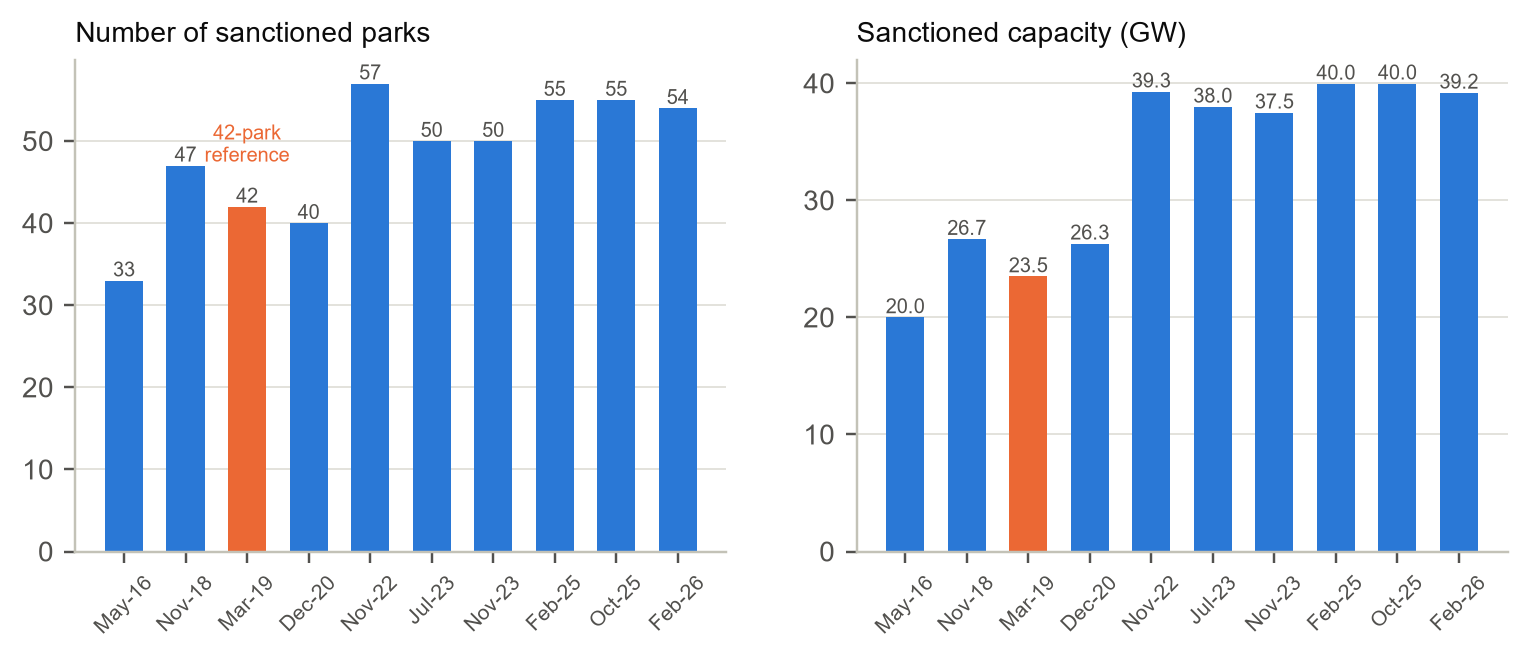
\includegraphics[width=0.85\textwidth]{timeline.png}
    \caption{Official number of sanctioned parks and sanctioned capacity at each reporting date. Orange marks the 42-park reference of March 2019.}
    \label{fig:timeline}
\end{figure}

The park-by-park list of the 42 parks of 2019 could not be retrieved: the relevant annexure of the MNRE Annual Report 2018--19 was not accessible during our research. We did not invent entries to reach 42. Instead we adopted the following, academically defensible definition:
\begin{itemize}[noitemsep]
    \item \textbf{Historical reference set:} 42 parks, 23,499~MW (31 March 2019), verified as a total.
    \item \textbf{Master universe:} the latest official park-wise list, 50 parks, 37,990~MW in 12 States (Lok Sabha Unstarred Question 3633, 10 August 2023) \cite{ls3633}.
    \item \textbf{Latest status:} 54 parks, 39,188~MW (February 2026) \cite{pibnote2026}.
\end{itemize}

\section{Master Solar Park Table}
\vspace{1mm}
Table~\ref{tab:master} lists all 50 parks. Names and sanctioned capacities come from the Lok Sabha answer. Commissioned capacity was reconstructed park by park from PIB data and reproduces the official totals exactly (10,237~MW; 11 complete and 7 partial parks) \cite{pib1941144, pib1983203}. Developers and approval dates come from the 2016 PIB Fact Sheet and SECI's park list. Coordinates are approximate, geocoded with OpenStreetMap from the officially named location; five parks have no verified location. The last column is the generation-data class defined in Section~3.7.

{\scriptsize
\setlength{\tabcolsep}{3pt}
\begin{longtable}{lp{3.6cm}p{1.9cm}rrrrp{1.6cm}lc}
\caption{Master table of the 50 MNRE-sanctioned solar parks (official park-wise list of 10 August 2023).}\label{tab:master}\\
\toprule
ID & Solar park & State & Lat & Long & Sanc. MW & Comm. MW & SPPD & Status & Data \\
\midrule
\endfirsthead
\toprule
ID & Solar park & State & Lat & Long & Sanc. MW & Comm. MW & SPPD & Status & Data \\
\midrule
\endhead
P01 & Ananthapuramu-I Solar Park (NP Kunta) & Andhra Pradesh & 14.05 & 78.41 & 1,400 & 1,400 & APSPCL & Complete & B \\
P02 & Kurnool Ultra Mega Solar Park & Andhra Pradesh & 15.67 & 78.29 & 1,000 & 1,000 & APSPCL & Complete & B \\
P03 & Kadapa Solar Park & Andhra Pradesh & 14.91 & 78.29 & 1,000 & 250 & APSPCL & Partial & B \\
P04 & Ananthapuramu-II Solar Park & Andhra Pradesh & 14.91 & 78.01 & 500 & 500 & APSPCL & Complete & B \\
P05 & Ramagiri Solar Park & Andhra Pradesh & 14.31 & 77.51 & 300 & 0 & Not verified & Under impl. & C \\
P06 & Rajnandgaon Solar Park & Chhattisgarh & 21.07 & 80.80 & 100 & 0 & CREDA & Under impl. & C \\
P07 & Radhnesada Solar Park & Gujarat & 24.36 & 71.51 & 700 & 500 & GPCL & Partial & B \\
P08 & Dholera Solar Park & Gujarat & 22.25 & 72.20 & 1,000 & 300 & GPCL & Partial & B \\
P09 & NTPC RE Park & Gujarat & 24.11 & 69.37 & 4,750 & 0 & NTPC & Under impl. & C \\
P10 & GSECL RE Park & Gujarat & 24.11 & 69.37 & 3,325 & 0 & GSECL & Under impl. & C \\
P11 & GIPCL RE Park Ph-I & Gujarat & 24.11 & 69.37 & 600 & 0 & GIPCL & Under impl. & C \\
P12 & GIPCL RE Park Ph-II & Gujarat & 24.11 & 69.37 & 1,200 & 0 & GIPCL & Under impl. & C \\
P13 & GIPCL RE Park Ph-III & Gujarat & 24.11 & 69.37 & 575 & 0 & GIPCL & Under impl. & C \\
P14 & SECI Floating Solar Park & Jharkhand & 23.45 & 85.55 & 100 & 0 & SECI & Under impl. & C \\
P15 & DVC Floating Solar Park Ph-I & Jharkhand & 23.84 & 86.81 & 755 & 0 & DVC & Dropped & D \\
P16 & DVC Floating Solar Park Ph-II & Jharkhand & 23.68 & 86.75 & 234 & 0 & DVC & Under impl. & C \\
P17 & Pavagada Solar Park & Karnataka & 14.24 & 77.42 & 2,000 & 2,000 & KSPDCL & Complete & B \\
P18 & Kalaburagi Solar Park & Karnataka & 17.24 & 76.77 & 500 & 0 & Not verified & Dropped & D \\
P19 & Kasargod Solar Park & Kerala & 12.37 & 75.13 & 105 & 100 & RPCKL & Partial & B \\
P20 & Kerala Floating Solar Park & Kerala & -- & -- & 50 & 0 & Not verified & Under impl. & C \\
P21 & Rewa Ultra Mega Solar Park & Madhya Pradesh & 24.47 & 81.55 & 750 & 750 & RUMSL & Complete & B \\
P22 & Mandsaur Solar Park & Madhya Pradesh & 24.26 & 75.39 & 250 & 250 & RUMSL & Complete & B \\
P23 & Neemuch Solar Park & Madhya Pradesh & 24.63 & 75.18 & 500 & 0 & RUMSL & Under impl. & C \\
P24 & Agar Solar Park & Madhya Pradesh & 23.72 & 76.02 & 550 & 0 & RUMSL & Under impl. & C \\
P25 & Shajapur Solar Park & Madhya Pradesh & 23.42 & 76.61 & 450 & 0 & RUMSL & Under impl. & C \\
P26 & Omkareshwar Floating Solar Park & Madhya Pradesh & 22.24 & 76.16 & 600 & 0 & RUMSL & Under impl. & C \\
P27 & Chhatarpur Solar Park & Madhya Pradesh & 24.76 & 79.68 & 950 & 0 & RUMSL & Under impl. & C \\
P28 & Barethi Solar Park & Madhya Pradesh & 24.78 & 79.72 & 630 & 0 & NTPC & Under impl. & C \\
P29 & Sai Guru Solar Park & Maharashtra & 20.99 & 74.32 & 500 & 0 & Sai Guru MSP & Under impl. & C \\
P30 & Dondaicha Solar Park & Maharashtra & 21.33 & 74.56 & 250 & 0 & MAHAGENCO & Under impl. & C \\
P31 & Vankal Solar Park & Mizoram & 23.52 & 93.19 & 20 & 20 & P\&E Dept. & Complete & B \\
P32 & Odisha Solar Park by NHPC & Odisha & -- & -- & 40 & 0 & NHPC & Under impl. & C \\
P33 & Odisha Floating Solar Park Ph-I & Odisha & -- & -- & 100 & 0 & Not verified & Dropped & D \\
P34 & Odisha Floating Solar Park Ph-II & Odisha & -- & -- & 200 & 0 & Not verified & Dropped & D \\
P35 & Bhadla-II Solar Park & Rajasthan & 27.54 & 71.92 & 680 & 680 & RSDCL & Complete & B \\
P36 & Bhadla-III Solar Park & Rajasthan & 27.54 & 71.92 & 1,000 & 1,000 & SUCRL & Complete & B \\
P37 & Bhadla-IV Solar Park & Rajasthan & 27.54 & 71.92 & 500 & 500 & AREPRL & Complete & B \\
P38 & Phalodi-Pokaran Solar Park & Rajasthan & 27.08 & 72.58 & 750 & 300 & ESUCRL & Partial & B \\
P39 & Fatehgarh Phase-1B Solar Park & Rajasthan & 26.49 & 71.21 & 421 & 421 & AREPRL & Complete & B \\
P40 & Nokh Solar Park & Rajasthan & 27.56 & 72.25 & 925 & 0 & RSDCL & Under impl. & C \\
P41 & Pugal Solar Park Ph-I & Rajasthan & 28.51 & 72.81 & 1,000 & 0 & Not verified & Under impl. & C \\
P42 & Pugal Solar Park Ph-II & Rajasthan & 28.51 & 72.81 & 1,000 & 0 & Not verified & Under impl. & C \\
P43 & RVUN Solar Park & Rajasthan & -- & -- & 2,000 & 0 & RVUNL & Under impl. & C \\
P44 & Solar Park in UP (LSPDCL) & Uttar Pradesh & 26.10 & 79.39 & 365 & 240 & LSPDCL & Partial & B \\
P45 & Jalaun Solar Park & Uttar Pradesh & 25.94 & 79.42 & 1,200 & 0 & BSUL & Under impl. & C \\
P46 & Mirzapur Solar Park & Uttar Pradesh & 24.93 & 82.63 & 100 & 0 & Not verified & Under impl. & C \\
P47 & Kalpi Solar Park & Uttar Pradesh & 26.12 & 79.75 & 65 & 26 & Not verified & Partial & B \\
P48 & Lalitpur Solar Park & Uttar Pradesh & 24.70 & 78.52 & 600 & 0 & Not verified & Under impl. & C \\
P49 & Jhansi Solar Park & Uttar Pradesh & 25.53 & 78.65 & 600 & 0 & Not verified & Under impl. & C \\
P50 & Chitrakoot Solar Park & Uttar Pradesh & 25.22 & 81.10 & 800 & 0 & Not verified & Under impl. & C \\
\hline
 & \textbf{Total (50 parks)} & 12 States & & & \textbf{37,990} & \textbf{10,237} & & & \\
\bottomrule

\end{longtable}
}

\section{Geographic Distribution}
\vspace{1mm}
The parks span from about 9.9$^\circ$N (Kasaragod, Kerala) to 28.5$^\circ$N (Pugal, Rajasthan) and from 69.4$^\circ$E (Khavda, Gujarat) to 93.2$^\circ$E (Vankal, Mizoram), as shown in Figure~\ref{fig:map}. They fall into five natural clusters: the Thar/Kutch desert cluster; the semi-arid Rayalaseema and south Karnataka cluster; central India; the Bundelkhand and Indo-Gangetic cluster; and single sites on the humid coast (Kasaragod), in the north-eastern hills (Vankal) and on reservoirs (floating parks). All five Grid-India regions are represented.

\begin{figure}[htbp]
    \centering
    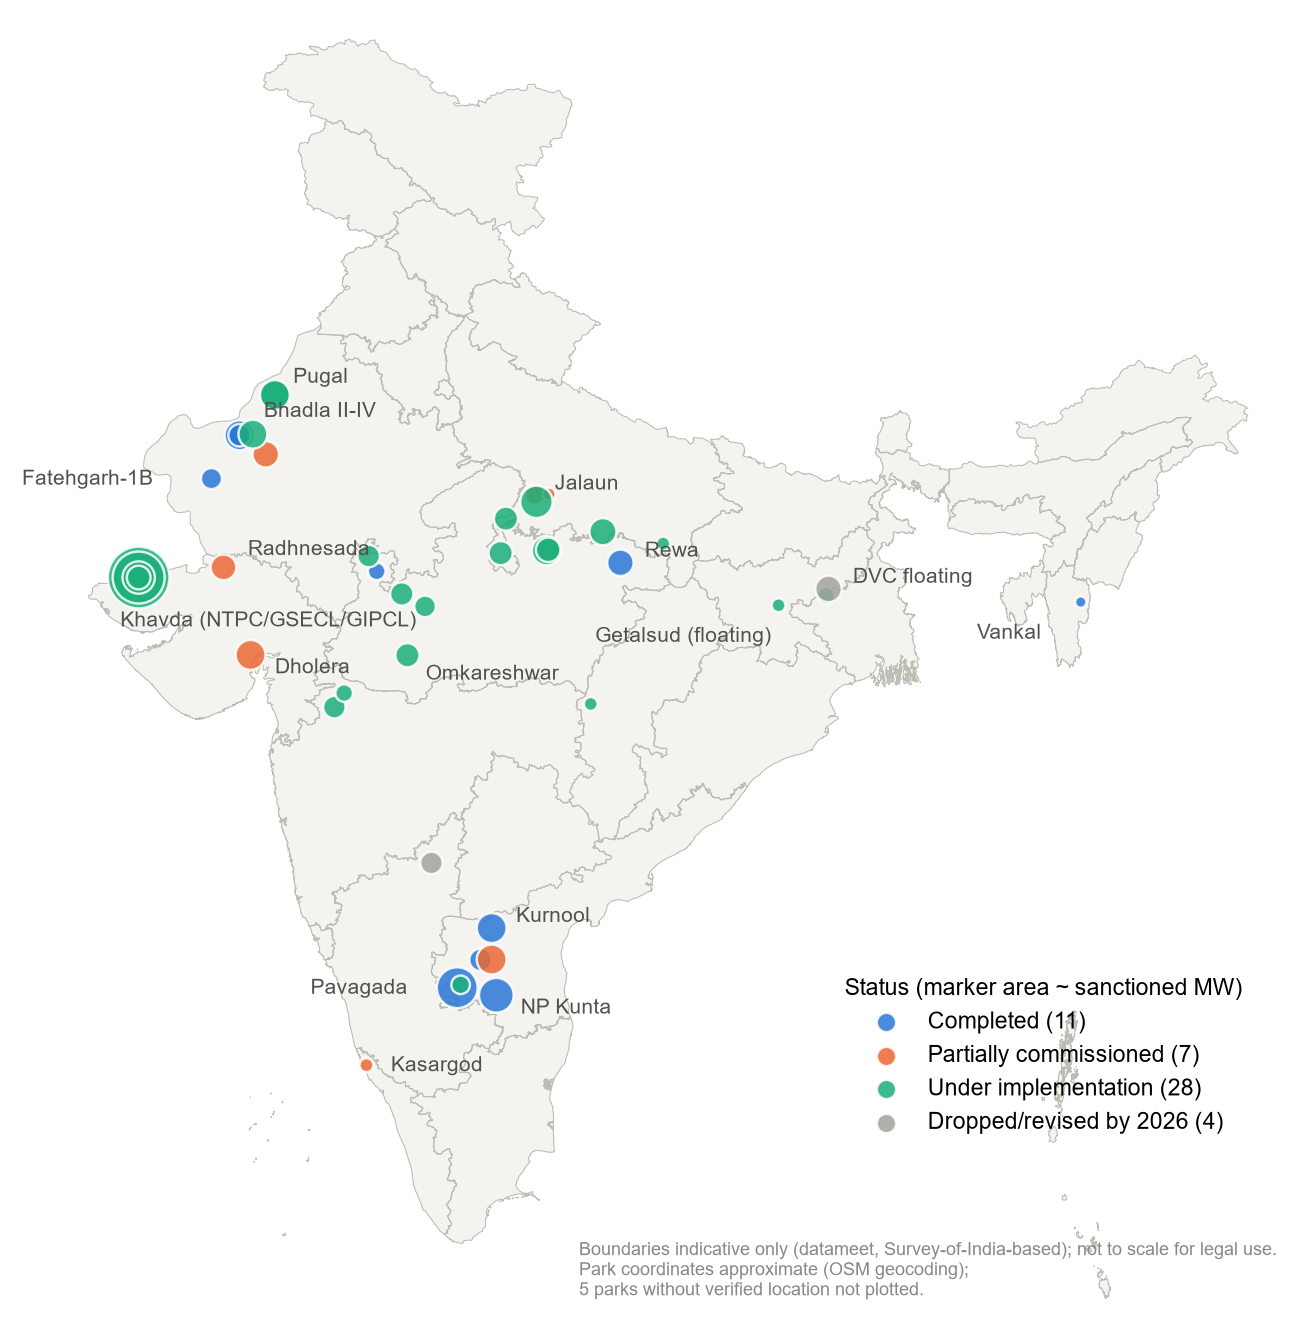
\includegraphics[width=0.62\textwidth]{map.png}
    \caption{Locations of the parks with a verified location, coloured by status; marker area is proportional to sanctioned capacity. Boundaries are indicative only.}
    \label{fig:map}
\end{figure}

\section{Capacity and Status}
\vspace{1mm}
Sanctioned capacity ranges from 20~MW (Vankal) to 4,750~MW (NTPC RE Park at Khavda), a ratio of more than 200. Gujarat and Rajasthan together hold 54\% of sanctioned capacity, while commissioned capacity in 2023 was led by Andhra Pradesh, Rajasthan and Karnataka (Figure~\ref{fig:statecap}). This wide range of sizes is the main reason we forecast output as a fraction of capacity (Section~5.3). As of August 2023, 11 parks were complete, 7 partially commissioned and 28 under implementation; 4 have since been dropped or revised. By October 2025, 14,922~MW of projects had been installed in the parks \cite{pib2199729}.

\begin{figure}[htbp]
    \centering
    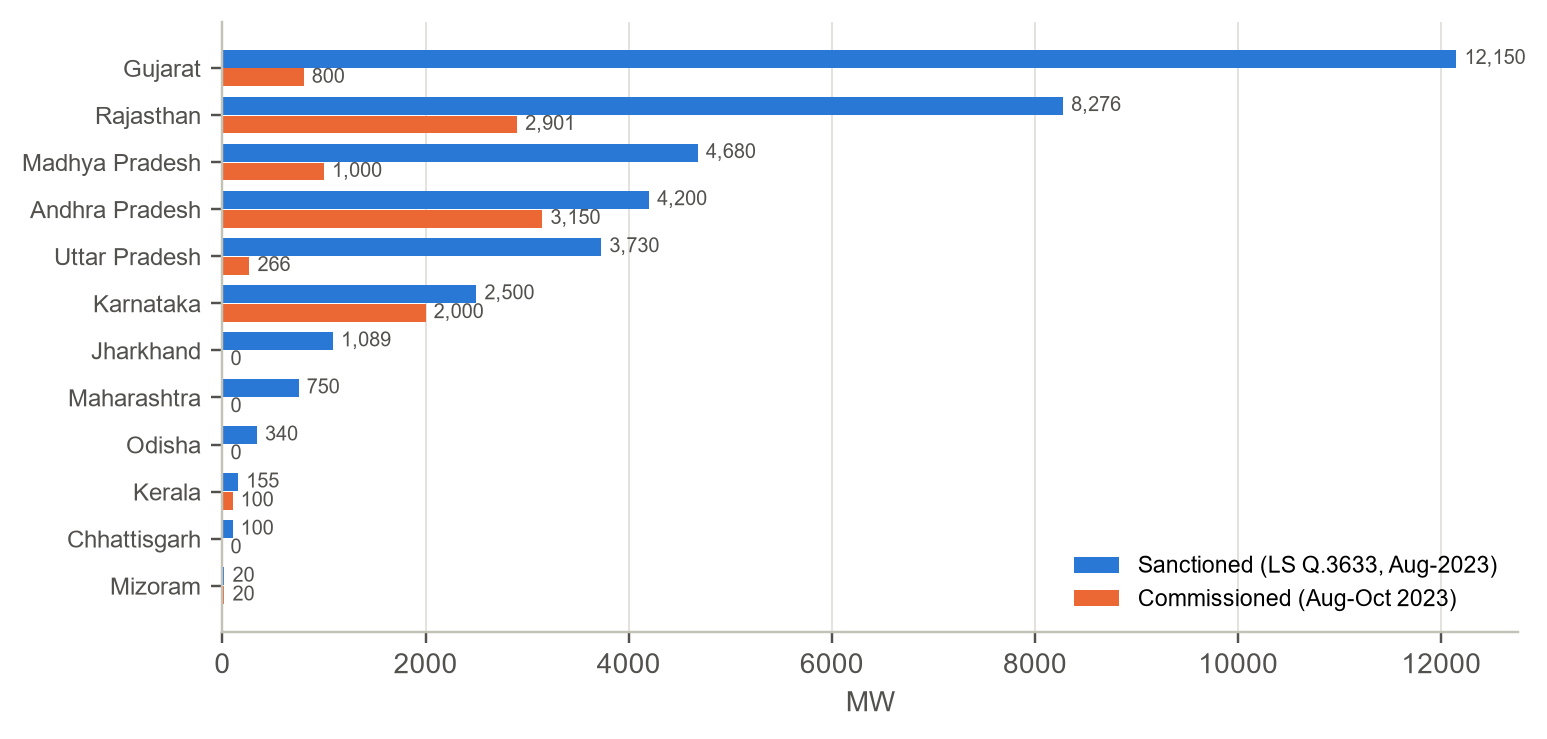
\includegraphics[width=0.78\textwidth]{state_capacity.png}
    \caption{Sanctioned and commissioned capacity by State (master universe).}
    \label{fig:statecap}
\end{figure}


\section{Data Availability Assessment}
\vspace{1mm}
We classified each park by the public availability of generation data:
\begin{itemize}[noitemsep]
    \item \textbf{Class A} -- actual hourly (or finer) generation publicly available: \textbf{0 parks}.
    \item \textbf{Class B} -- partial: commissioned and generating, with official cumulative figures; plant-level schedules or daily energy may exist in load-despatch or developer publications: \textbf{18 parks}.
    \item \textbf{Class C} -- capacity and commissioning information only: \textbf{28 parks}.
    \item \textbf{Class D} -- insufficient data, or dropped/revised by 2026: \textbf{4 parks}.
\end{itemize}
The absence of any Class-A park is the central practical constraint of the project and motivates the generation-data strategy in Chapter~5.

% ================================================================ 4
\chapter{Literature Review and Research Gap}
This chapter summarises relevant work on solar power forecasting and identifies the gap that our project addresses.

\section{Review of Solar Forecasting Research}
\vspace{1mm}
Solar forecasting has grown rapidly over the last fifteen years. Antonanzas et al.\ \cite{antonanzas2016} reviewed photovoltaic power forecasting and concluded that machine-learning methods driven by NWP inputs dominate for horizons of hours to a day, while persistence remains a hard-to-beat reference for very short horizons. Yang et al.\ \cite{yang2018} analysed the literature by text mining and stressed the importance of proper baselines (especially clear-sky persistence), standard metrics and honest validation.

\subsubsection{Tree-based ensembles}
Random Forests \cite{breiman2001}, XGBoost \cite{xgboost} and LightGBM \cite{lightgbm} handle tabular weather and time features well. They train quickly, need little data preparation and provide feature-importance measures. LightGBM in particular scales to millions of rows and supports quantile objectives for interval forecasts.

\subsubsection{Deep learning}
Recurrent networks such as LSTM \cite{lstm} and GRU \cite{gru} learn temporal patterns directly from sequences. More recent architectures, such as the Temporal Fusion Transformer \cite{tft} and N-HiTS \cite{nhits}, handle known future inputs (such as NWP forecasts) and multiple related series. For NWP-driven tabular problems, however, gradient boosting often matches or beats deep models at much lower cost.

\subsubsection{Multi-site and spatial forecasting}
Global models trained on many sites share information between them and can forecast sites with little history. Aggregating many geographically spread plants smooths variability because cloud effects at distant sites are weakly correlated \cite{hoff2010}. Graph neural networks have been proposed to exploit spatial structure explicitly.

\subsubsection{Uncertainty quantification}
Quantile regression \cite{koenker1978} and conformal prediction \cite{romano2019} are practical ways to produce prediction intervals. Adaptive conformal inference \cite{gibbs2021} adjusts the intervals when the data distribution shifts, for example between seasons.

\section{Research Gap}
\vspace{1mm}
Based on our review, five gaps are relevant to India:
\begin{enumerate}[noitemsep]
    \item \textbf{Single-site focus.} Indian studies usually forecast one plant with a proprietary or short dataset. Benchmarks across the officially documented solar park portfolio are scarce.
    \item \textbf{Missing generation data.} Few studies address how to forecast a portfolio where most sites have no public measurements, or how large the gap is between simulated and real output.
    \item \textbf{Generalisation to new parks.} Per-park, global and regional models, and their performance on parks not seen in training, are rarely compared across Indian climates.
    \item \textbf{Aggregation.} The smoothing benefit of aggregating Indian solar parks, and the calibration of intervals at aggregate levels, are seldom measured.
    \item \textbf{Over-optimistic validation.} Many studies feed models the weather that actually occurred (reanalysis or measurements) as if it had been known in advance. This overstates accuracy. Archived NWP forecasts give a realistic picture.
\end{enumerate}
We do not claim to be the first to do multi-site solar forecasting. Our contribution is a reproducible, officially sourced, honestly validated benchmark for Indian solar parks.

\section{Research Questions}
\vspace{1mm}
\textbf{Central question:} Can a single, capacity-normalised, weather-aware machine-learning framework, driven by archived numerical weather forecasts, produce accurate and well-calibrated short-term solar generation forecasts across India's geographically diverse MNRE-sanctioned solar parks, including parks without measured history?

\begin{table}[htbp]
\centering
\caption{Research questions and the experiments that answer them.}
\label{tab:rq}
\begin{tabularx}{\textwidth}{lLl}
\toprule
RQ & Question & Experiment \\
\midrule
RQ1 & Which model family performs best, and is the difference significant? & E1 \\
RQ2 & How does accuracy vary across climatic regions and seasons? & E1--E3 \\
RQ3 & How much do irradiance, clouds, temperature and lagged generation contribute? & E4 \\
RQ4 & Does aggregation reduce capacity-normalised error? & E5 \\
RQ5 & How accurately are ramp events forecast? & E6 \\
RQ6 & Can one global model match per-park and regional models? & E2, E3 \\
RQ7 & Are conformal prediction intervals well calibrated? & E8 \\
RQ8 & Can a global model forecast parks it has never seen? & E7 \\
RQ9 & How much accuracy is lost with realistic NWP instead of oracle weather? & E9 \\
RQ10 & How large is the simulation-to-reality gap? & E10 \\
\bottomrule
\end{tabularx}
\end{table}

% ================================================================ 5
\chapter{Methodology}
This chapter describes the data sources, the strategy for missing generation data, the physical simulation, feature engineering, models, multi-site designs, aggregation, ramp analysis, uncertainty quantification, validation and evaluation metrics. 


\section{Data Sources}
\vspace{1mm}
We compared several weather and irradiance sources for coverage, resolution, history, cost and ease of access (Table~\ref{tab:weather}).

\begin{table}[htbp]
\centering
\caption{Comparison of weather and irradiance data sources.}
\label{tab:weather}
\footnotesize
\begin{tabularx}{\textwidth}{p{2.5cm}p{3.0cm}p{2.3cm}LL}
\toprule
Source & Resolution & History & Access & Role in project \\
\midrule
ERA5 \cite{era5} & 0.25$^\circ$, hourly & 1940--present & Free (Copernicus / Open-Meteo) & Observed weather for targets \\
ERA5-Land \cite{era5land} & 0.1$^\circ$, hourly & 1950--present & Free & Higher-resolution check (no cloud cover) \\
ECMWF IFS archived forecasts & 0.25$^\circ$, hourly & Mar 2024--present & Free via Open-Meteo Previous Runs API \cite{openmeteo} & Forecast features (model inputs) \\
NASA POWER \cite{nasapower} & $\sim$1$^\circ$ solar, hourly & 2001--present & Free REST API & Independent cross-check \\
CAMS radiation \cite{cams} & Satellite, 1-min to monthly & 2004--present & Free with registration & Irradiance validation where covered \\
IMD / MOSDAC & Stations, satellite products & Varies & Registration, partly restricted & Optional validation \\
Solcast & Satellite-based & 2007--present & Commercial & Not used (cost) \\
\bottomrule
\end{tabularx}
\end{table}

Our final choice uses only free sources:
\begin{itemize}[noitemsep]
    \item \textbf{Park metadata:} MNRE, PIB, Lok Sabha and Rajya Sabha answers, SECI.
    \item \textbf{Observed weather (targets):} ERA5 reanalysis via the Open-Meteo Historical Weather API.
    \item \textbf{Forecast weather (features):} ECMWF IFS 0.25$^\circ$ archived forecasts via the Open-Meteo Previous Runs API, using the forecasts issued one day (\texttt{previous\_day1}) and two days (\texttt{previous\_day2}) before each valid time.
    \item \textbf{Locations:} OpenStreetMap geocoding of the officially named park location.
\end{itemize}

\section{Generation Data Strategy}
\vspace{1mm}
Five strategies were evaluated:
\begin{itemize}[noitemsep]
    \item \textbf{A -- Actual generation:} ground truth, but unavailable for almost all parks.
    \item \textbf{B -- Physical PV modelling:} available for every park and hour, but depends on assumptions and contains no operational effects.
    \item \textbf{C -- Hybrid:} actual data where available, simulated elsewhere, with a source flag on every row. \textbf{Adopted.}
    \item \textbf{D -- Transfer learning:} pre-train on simulated or data-rich parks and fine-tune on measured parks. Tested on two real plants in experiment E11.
    \item \textbf{E -- Normalised forecasting:} forecast output as a fraction of capacity. \textbf{Adopted.}
\end{itemize}

\section{Normalised Target}
\vspace{1mm}
Instead of forecasting megawatts directly, we forecast normalised power:
\begin{equation}
    p_i(t) = \frac{P_i(t)}{C_i(t)}
\end{equation}
where $P_i(t)$ is the AC output of park $i$ and $C_i(t)$ its commissioned AC capacity. The MW forecast is recovered as
\begin{equation}
    \hat{P}_i(t+h) = \hat{p}_i(t+h) \times C_i(t+h)
\end{equation}
This puts a 20~MW and a 4,750~MW park on the same scale, so one global model can learn the weather-to-power relation once and apply it everywhere. Two conditions apply: $C_i(t)$ must be the commissioned capacity at time $t$, not the sanctioned capacity; and differences that normalisation does not remove (DC/AC ratio, trackers, floating installations) must be given to the model as metadata.

\section{Physical PV Simulation}
\vspace{1mm}
Targets are simulated with \texttt{pvlib} \cite{pvlib} using the chain described in Section~2.3. The assumptions are listed in Table~\ref{tab:pvassump}. All of them are reported as assumptions.

\begin{table}[htbp]
\centering
\caption{PV simulation assumptions.}
\label{tab:pvassump}
\begin{tabularx}{\textwidth}{p{3.2cm}Lp{4.2cm}}
\toprule
Component & Setting & Note \\
\midrule
Solar position & NREL SPA, at mid-interval & Exact \\
Clear-sky model & Ineichen with Linke turbidity & For normalisation \\
Transposition & Perez \cite{perez1990} & Albedo 0.20 (0.25 desert) \\
Mounting & Fixed tilt = latitude, south facing; floating 10$^\circ$ & Trackers not modelled \\
Cell temperature & SAPM open rack (ground); Faiman $u_0{=}35$, $u_1{=}8$ (floating) & Floating cooled by water \\
DC model & PVWatts, $\gamma = -0.37$\%/$^\circ$C & Crystalline silicon \\
DC/AC ratio & 1.25 & Causes noon clipping \\
Losses & PVWatts default 14.08\%; soiling 4\% in Rajasthan and Gujarat & Dust in Thar/Kutch \\
Inverter & PVWatts, 96\% efficiency, clipped at AC rating & -- \\
\bottomrule
\end{tabularx}
\end{table}

\textbf{Avoiding circular targets.} If the target were simulated from the same weather that the model receives as input, the model could simply learn to imitate \texttt{pvlib} and appear almost perfect. We therefore separate the two: \textbf{targets} are simulated from ERA5 \textit{observed} weather at the valid time, while \textbf{features} are ECMWF \textit{forecasts} issued earlier. The forecast error of the model then reflects real weather-forecast error, as in operations.

\section{Feature Engineering}
\vspace{1mm}
All features must be available at the forecast issue time $t$. The feature groups are:
\begin{itemize}[noitemsep]
    \item \textbf{Time:} hour, day of year, month and season, with cyclical encoding:
    \begin{equation}
        h_{sin} = \sin\!\left(\frac{2\pi\,\text{hour}}{24}\right),\quad h_{cos} = \cos\!\left(\frac{2\pi\,\text{hour}}{24}\right)
    \end{equation}
    and similarly for day of year with period 365.25.
    \item \textbf{Historical power:} $p(t)$, $p(t-1)$, $p(t-2)$, $p(t-3)$, $p(t-6)$, $p(t-24)$.
    \item \textbf{Rolling statistics:} 3, 6 and 24-hour means and standard deviations.
    \item \textbf{Forecast weather at $t+h$:} GHI, DNI, DHI, temperature, cloud cover, humidity, pressure, wind speed, precipitation.
    \item \textbf{Solar geometry at $t+h$:} zenith, elevation, azimuth, angle of incidence, clear-sky irradiance.
    \item \textbf{Physics feature:} \texttt{pvlib} power computed from the NWP forecast, so that the ML model learns a correction to physics.
    \item \textbf{Park metadata:} latitude, longitude, elevation, capacity, State, grid region, climate class, mounting type, park identifier.
\end{itemize}

\section{Forecasting Horizons}
\vspace{1mm}
The forecast horizons are $t+1$, $t+3$, $t+6$ and $t+24$ (day-ahead) hours at hourly resolution. A \textit{direct} strategy is used (one model per horizon, or the horizon as a feature) to avoid the error build-up of recursive forecasting. Night hours are excluded from normalised metrics (daylight is defined as solar elevation above 5$^\circ$). The forecasts used as inputs must have been available at time $t$. A forecast from the \texttt{previous\_day1} series was issued about 24 hours before its valid time, so with about 6 hours of NWP latency it is usable for horizons up to 18 hours. Day-ahead forecasts use the \texttt{previous\_day2} series.

\section{Baseline Models}
\vspace{1mm}
\begin{itemize}[noitemsep]
    \item \textbf{Persistence:} $\hat{P}(t+h) = P(t)$.
    \item \textbf{Smart persistence:} $\hat{P}(t+h) = k(t)\,P_{cs}(t+h)$, the main baseline to beat.
    \item \textbf{Diurnal persistence:} $\hat{P}(t+h) = P(t+h-24)$.
    \item \textbf{Climatology:} mean output for the same park, month and hour.
    \item \textbf{Physical NWP forecast:} \texttt{pvlib} applied to the NWP forecast.
    \item \textbf{Linear regression:} a ridge model on the main features.
\end{itemize}
Model skill is measured against smart persistence:
\begin{equation}
    \text{Skill} = 1 - \frac{\text{RMSE}_{model}}{\text{RMSE}_{smart\ persistence}}
\end{equation}

\section{Machine-Learning and Deep-Learning Models}
\vspace{1mm}
\textbf{Machine learning:} Ridge regression, Random Forest, XGBoost \cite{xgboost} and CatBoost \cite{catboost} (both on the GPU) and \textbf{LightGBM} (primary). LightGBM is chosen as the main model because it is fast on about 1.6 million rows, handles the park identifier as a categorical feature, and supports quantile objectives. Hyper-parameters are tuned on the calibration period only (experiment E10). Feature importance (RQ3) is measured with SHAP values \cite{shap} and feature-group ablation.\\

\textbf{Deep learning:} LSTM and GRU networks with a 48-hour look-back window plus NWP inputs for the forecast horizon. Both networks are trained with PyTorch on the GPU. Larger networks (Temporal Fusion Transformer, N-HiTS) were left for future work, because LSTM and GRU did not beat LightGBM.

\section{Multi-Site Modelling Designs}
\vspace{1mm}
\begin{table}[htbp]
\centering
\caption{Multi-site modelling approaches.}
\label{tab:multisite}
\begin{tabularx}{\textwidth}{p{3cm}LL}
\toprule
Approach & Advantages & Disadvantages \\
\midrule
Per-park models & Capture site-specific behaviour & Need history at every park; cannot serve new parks \\
Global model & Shares learning; data-efficient; serves unseen parks & May underfit unusual sites (floating, hills) \\
Regional models & Climate-consistent training data & Groupings must be justified; small regions have little data \\
Global + fine-tuning & Combines both; tests transfer & More complex; risk of overfitting \\
\bottomrule
\end{tabularx}
\end{table}
Regions are defined in three objective ways: Grid-India regions (operational), Köppen--Geiger climate classes from the 1-km map of Beck et al.\ \cite{beck2018}, and data-driven clusters of monthly weather statistics.

\section{Aggregated Forecasting}
\vspace{1mm}
Park forecasts are summed to four levels:
\begin{equation}
    \hat{P}_{state} = \sum_{i \in state} \hat{P}_i, \qquad \hat{P}_{region} = \sum_{s \in region} \hat{P}_s, \qquad \hat{P}_{total} = \sum_i \hat{P}_i
\end{equation}
The variance of the aggregate error is $\sum_i \sigma_i^2 + 2\sum_{i<j}\rho_{ij}\sigma_i\sigma_j$. When the error correlation $\rho_{ij}$ falls with distance, the aggregate error grows more slowly than capacity, which is the smoothing effect \cite{hoff2010}. We measure $\rho_{ij}$ against distance and compare nRMSE at each level. Prediction intervals are calibrated separately at each level, because quantiles cannot simply be added.


\section{Ramp Event Analysis}
\vspace{1mm}
Because sunrise and sunset changes are predictable, ramps are defined on normalised quantities:
\begin{equation}
    r(t) = \frac{P(t) - P(t-1)}{C(t)}, \qquad \Delta k(t) = k(t) - k(t-1)
\end{equation}
A ramp event is flagged when $|\Delta k(t)| > 0.3$ and clear-sky power exceeds 10\% of capacity, or when $|r(t)|$ exceeds the 95th percentile at that park. Errors are compared between ramp and non-ramp hours and across weather regimes (clear, partly cloudy, overcast, monsoon, extreme heat), using MAE and event-detection scores (probability of detection, false-alarm ratio, critical success index).

\section{Uncertainty Quantification}
\vspace{1mm}
We train LightGBM quantile models (10th, 50th and 90th percentiles) and calibrate them with conformalised quantile regression (CQR) \cite{romano2019} on the July--December 2025 calibration period. For the all-parks total, a split-conformal interval is fitted directly on the summed forecast. Intervals are evaluated with prediction interval coverage probability (PICP) and mean normalised width.

\section{Validation Methodology}
\vspace{1mm}
Time series must never be randomly shuffled, because future information would leak into training. We use (Figure~\ref{fig:valsplit}):
\begin{itemize}[noitemsep]
    \item \textbf{Chronological split:} train April 2024--June 2025, calibration/validation July--December 2025, test January--September 2026. Each part contains a monsoon period.
    \item \textbf{One untouched test period:} models are fitted on the training period, with early stopping and calibration on the second period, and see the test period only once.
    \item \textbf{Leave-one-park-out / leave-one-location-out} to test generalisation. Parks that share a weather location (e.g.\ Bhadla II--IV) are held out together.
    \item \textbf{Fixed random seeds} and every result saved as a table, so all numbers can be reproduced.
\end{itemize}

\begin{figure}[htbp]
    \centering
    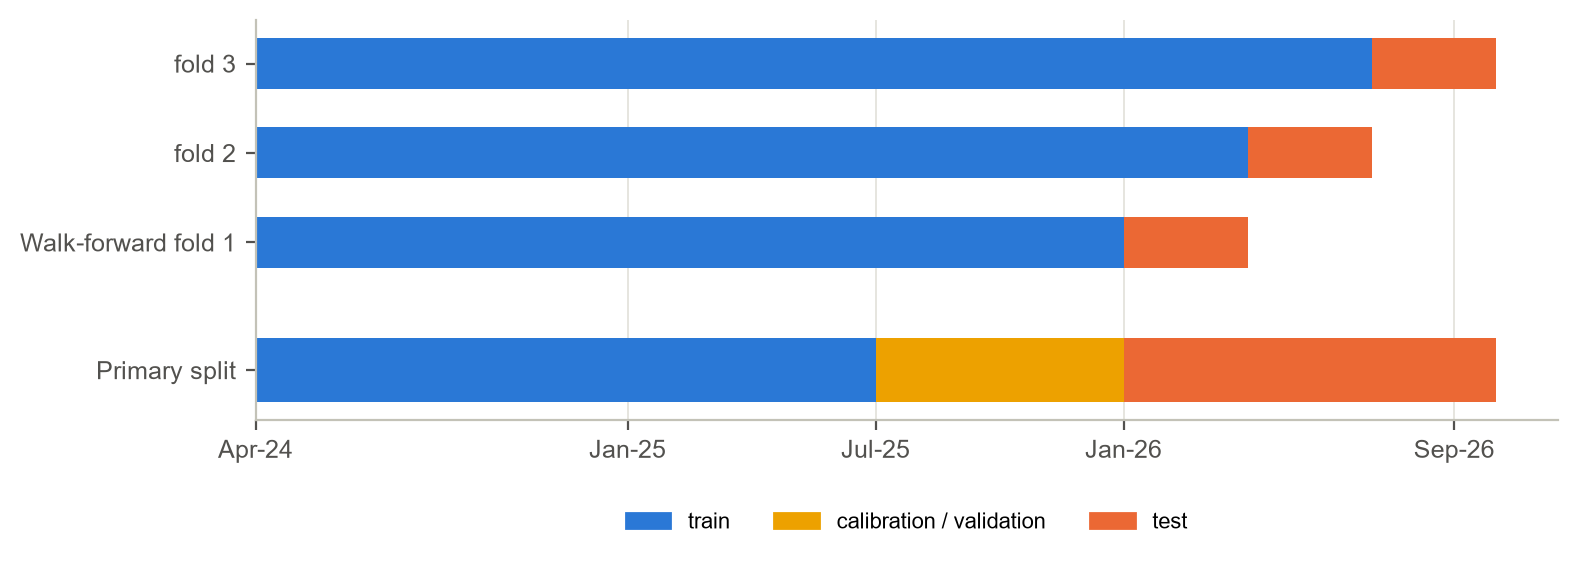
\includegraphics[width=0.85\textwidth]{validation_split.png}
    \caption{Chronological split and walk-forward folds (no shuffling).}
    \label{fig:valsplit}
\end{figure}

\section{Evaluation Metrics}
\vspace{1mm}
With $n$ daylight hours and capacity $C$:
\begin{align}
    \text{MAE} &= \frac{1}{n}\sum |P - \hat{P}| \\
    \text{RMSE} &= \sqrt{\frac{1}{n}\sum (P - \hat{P})^2} \\
    \text{nRMSE} &= \frac{\text{RMSE}}{C}\times 100\%, \qquad \text{nMAE} = \frac{\text{MAE}}{C}\times 100\% \\
    R^2 &= 1 - \frac{\sum (P - \hat{P})^2}{\sum (P - \bar{P})^2}
\end{align}
MAPE is computed only when $P > 0.1\,C$, because near sunrise, sunset and at night the denominator approaches zero and MAPE becomes meaningless.

\section{Experiments}
\vspace{1mm}
\begin{table}[htbp]
\centering
\caption{List of experiments.}
\label{tab:exp}
\begin{tabularx}{\textwidth}{lp{3.6cm}L}
\toprule
Exp. & Comparison & Design \\
\midrule
E1 & Persistence vs ML vs DL & All models, same features and splits, $h = 1, 3, 6, 24$ \\
E2 & Individual vs global & Per-park models vs one global LightGBM \\
E3 & Global vs regional & Grid-region, Köppen and weather-cluster models \\
E4 & Weather-only vs weather + history & Feature-group ablation and SHAP \\
E5 & Single park vs aggregated & nRMSE at four levels; error correlation vs distance \\
E6 & Normal vs ramp conditions & Errors stratified by ramp flag and weather regime \\
E7 & Seen vs unseen parks & Leave-one-location-out \\
E8 & Point vs interval forecast & Quantile LightGBM vs CQR \\
E9 & Oracle vs NWP inputs & Same model with reanalysis vs forecast inputs \\
E10 & Default vs tuned & CatBoost (GPU) and tuned LightGBM \\
E11 & Simulation-to-reality & Simulated-trained model tested on two measured plants \\
\bottomrule
\end{tabularx}
\end{table}

% ================================================================ 6
\chapter{System Architecture and Implementation}
This chapter describes the overall system architecture, the technology stack and the implementation: park registry, weather downloader, PV simulator, feature building and model training.

\section{System Architecture}
\vspace{1mm}
The system is organised in eight layers (Figure~\ref{fig:arch}): data sources; ingestion; target construction; data engineering; modelling; forecast products; uncertainty and evaluation; and serving. Compared with a simple single-site pipeline, it adds a park registry with a capacity timeline, a target-construction layer that records whether each value is measured or simulated, two separate weather streams (forecasts for features, reanalysis for targets), grid-region aggregation and a model registry that makes every dashboard forecast traceable to a model version.

\begin{figure}[htbp]
    \centering
    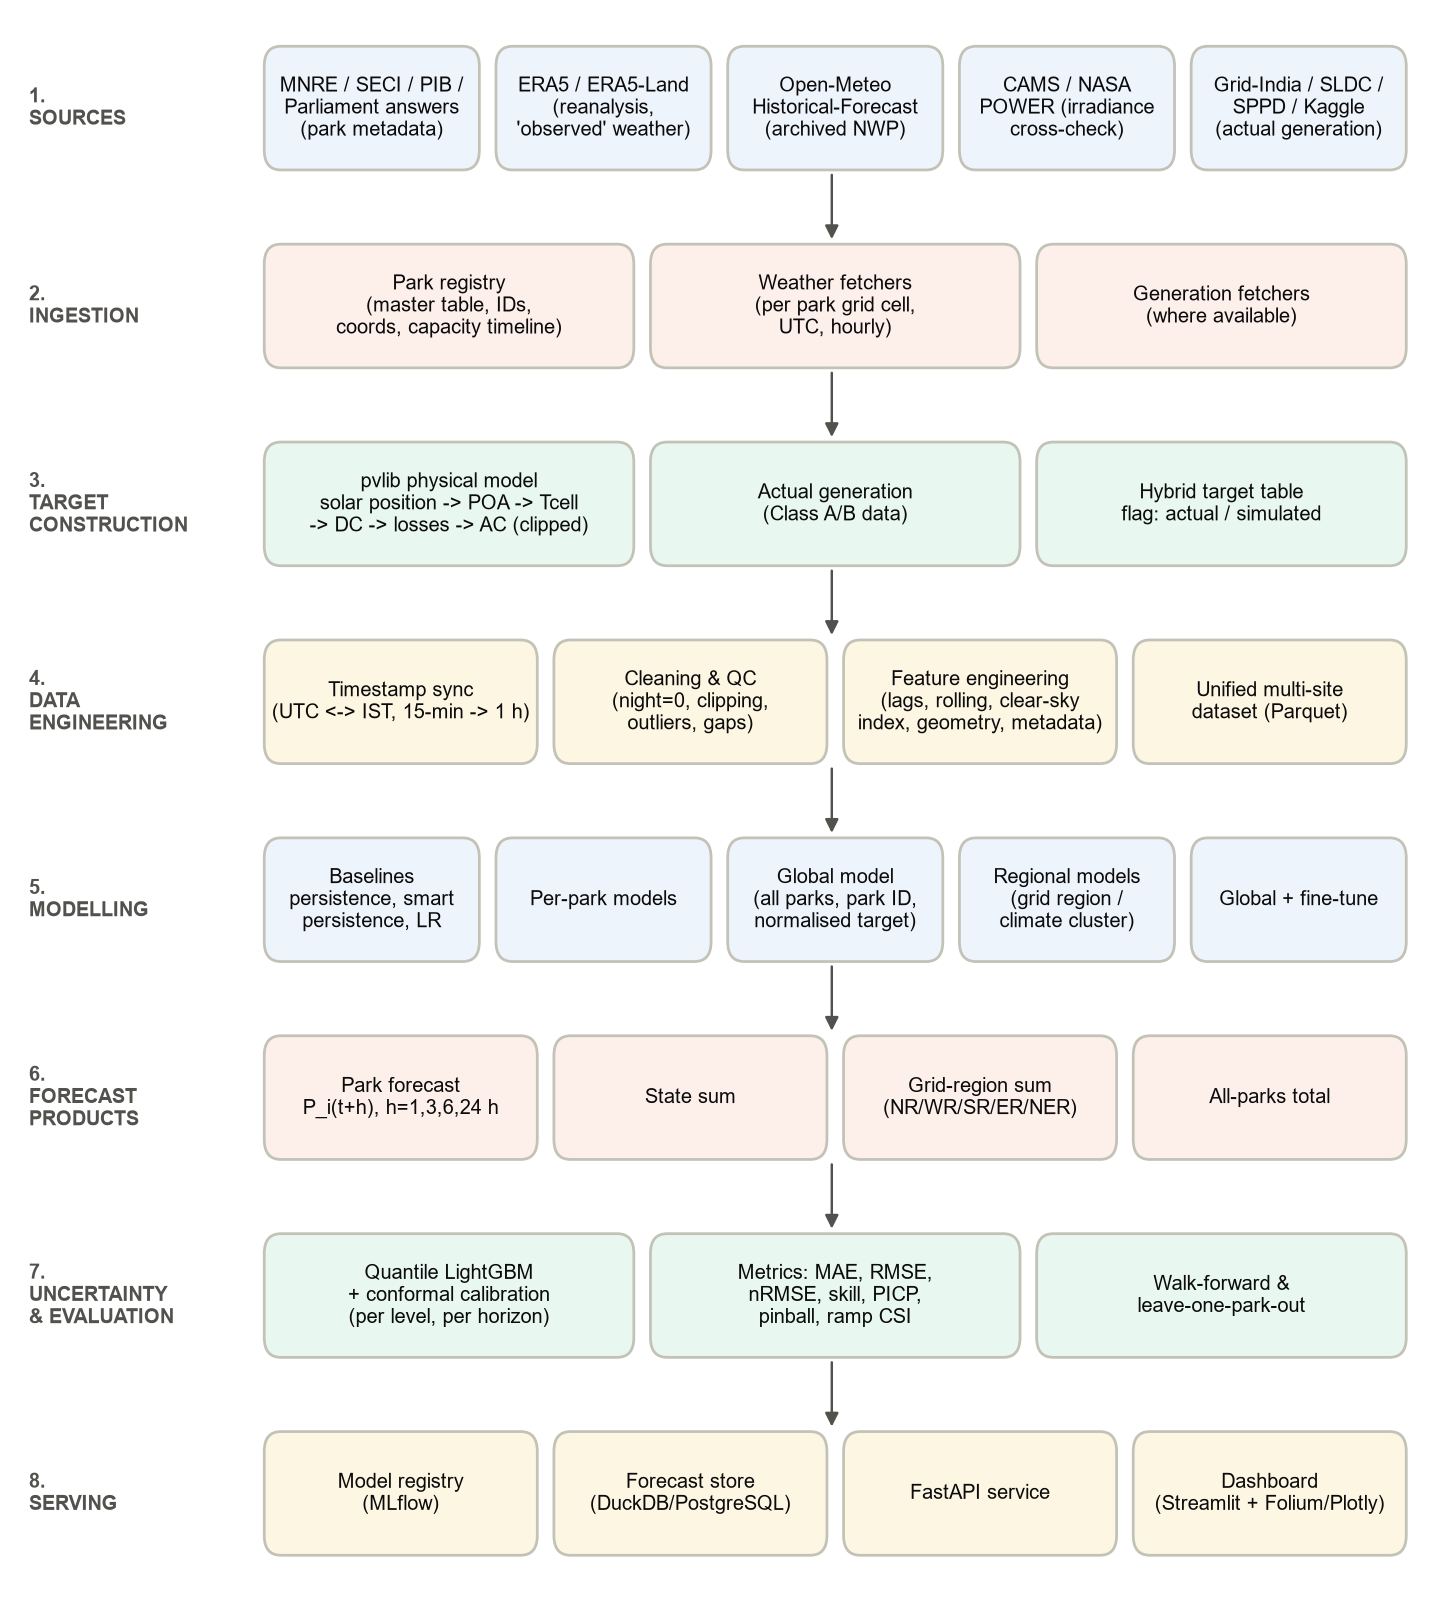
\includegraphics[width=0.62\textwidth]{architecture.png}
    \caption{Layered system architecture.}
    \label{fig:arch}
\end{figure}

\section{Technology Stack}
\vspace{1mm}
\begin{table}[htbp]
\centering
\caption{Technology stack.}
\label{tab:tech}
\begin{tabularx}{\textwidth}{p{3.4cm}Lp{4.4cm}}
\toprule
Layer & Tools & Reason \\
\midrule
Language & Python 3 & Scientific and ML ecosystem \\
Data access & requests, Open-Meteo APIs & Free weather data \\
Data processing & pandas, NumPy, PyArrow/Parquet & Fast, laptop-scale \\
Solar physics & pvlib & Validated open-source PV modelling \\
Machine learning & scikit-learn, LightGBM, XGBoost (CUDA), CatBoost (GPU), SHAP & Fast, well documented \\
Deep learning & PyTorch with CUDA (LSTM, GRU) & GPU training \\
Uncertainty & Own conformal (CQR) code & Transparent methods \\
Climate zones & kgcpy (Köppen--Geiger), k-means & Objective grouping \\
Charts and maps & Plotly, Matplotlib, Chart.js, SVG map & Maps and charts \\
Serving & FastAPI, Uvicorn & Lightweight API \\
Dashboard and website & Streamlit; static website on GitHub Pages & Free public hosting \\
Quality & pytest, Git & Testing, version control \\
\bottomrule
\end{tabularx}
\end{table}

\section{Project Structure}
\vspace{1mm}
The code is organised as a small Python package (\texttt{config}, \texttt{registry}, \texttt{openmeteo} and \texttt{pvsim} modules) driven by fourteen numbered scripts: build the park registry, download the weather, simulate the targets, quality control, build features, train the machine-learning models, run the experiments, train the deep-learning models, summarise the results, CatBoost and tuning, the real-data check, export the website data, climate grouping and build the public website. Each script can be rerun on its own. Unit tests and a design-decision log are kept alongside the code.

\section{Park Registry}
\vspace{1mm}
The registry converts the master table into modelling metadata. Each park is assigned a tier:
\begin{itemize}[noitemsep]
    \item \textbf{Core (U2):} commissioned capacity greater than zero, 18 parks, 10,237~MW. MW forecasts use commissioned capacity.
    \item \textbf{Virtual (U3):} under implementation, 25 parks with a verified location, simulated at sanctioned capacity and clearly flagged as virtual sites.
    \item \textbf{Excluded:} 7 parks (2 dropped or revised by 2026, 5 without a verified location).
\end{itemize}
Parks with identical coordinates share one weather location (Bhadla II--IV, the five Khavda parks and Pugal I--II), giving \textbf{43 modelled parks at 36 weather locations}. Floating parks are identified from their names and simulated with different mounting and cooling settings.

\section{Weather Downloader}
\vspace{1mm}
The downloader requests one calendar year of data per location and dataset and stores each chunk as a Parquet file with a metadata file (grid point, elevation, model, download time). Interrupted downloads resume automatically because cached chunks are skipped. A persistent, weighted rate limiter keeps usage within the free limits of the Open-Meteo service. Requests with more than 10 variables or more than two weeks of data count as several calls, so the limiter estimates the weight of each request before sending it. Network errors and server errors are retried with exponential back-off, and ``limit exceeded'' replies trigger a pause.\\

The full download covered 36 locations $\times$ 2 datasets $\times$ 3 yearly chunks = 216 requests, an estimated 6,689 weighted API calls, and completed in about two hours with no missing data.

\section{Key Design Decisions}
\vspace{1mm}
\subsubsection{Study window (April 2024 -- September 2026)}
Our scope document originally proposed 2022--2025. While implementing, we found that archived NWP forecasts with a known lead time are available from January 2024 for GFS and only from mid-March 2024 for ECMWF IFS at Indian locations. An older archive (the Historical Forecast API) goes back to 2022, but it stitches together the first hours of the most recent forecast run for each time. It can therefore contain information issued after the forecast issue time. We chose honesty over length and moved the window to April 2024 -- September 2026.

\subsubsection{Lead-time rule}
For issue time $t$ and horizon $h$, a forecast from the \texttt{previous\_dayN} series is usable only if $24N - h \geq 6$ hours. The day-1 series is used for horizons of 1--6 hours and the day-2 series for day-ahead forecasts. This is conservative: intraday skill must come from recent generation, as in real operations.

\subsubsection{Time convention}
All timestamps are UTC and mark the \textit{end} of the hour over which radiation is averaged. Solar geometry is computed at the middle of the interval ($t - 30$ minutes). IST (UTC+5:30) is used only for display and for seasons.

\section{PV Simulation Module}
\vspace{1mm}
The simulation module implements the chain of Section~2.3 with \texttt{pvlib}: Perez transposition, the ASHRAE incidence-angle modifier, SAPM (ground) or Faiman (floating) cell temperature, the PVWatts DC model, system losses and a clipped PVWatts inverter, giving output as a fraction of AC capacity. The same chain is also run with clear-sky irradiance to obtain clear-sky power, which is needed for smart persistence and for ramp detection.
Missing weather values produce missing (not zero) power, so gaps can never be mistaken for night or overcast conditions.

\section{Model Training}
\vspace{1mm}
For each horizon one table of about 1.6 million park-hours is built (one row per park and issue hour). The target is output as a fraction of capacity, so large and small parks can share one model. Only daylight hours are used for training and scoring. All models are trained on a laptop with an NVIDIA RTX 4060 GPU: XGBoost on the GPU takes 2--3 seconds per horizon, LightGBM under a minute on the CPU, and each LSTM or GRU about 20--30 seconds on the GPU. Each trained model's forecasts for the test period are saved, and the dashboard, API and website read these saved forecasts.

\section{Testing}
\vspace{1mm}
Nine automated tests check that the registry reproduces the official totals (50 parks, 37,990~MW sanctioned, 10,237~MW commissioned, 18 core parks); that co-located parks share a weather location; and that the simulator behaves physically (near-rated output at clear-sky noon, zero output at night, peak between 11:00 and 13:00 IST, lower output when cells are hotter, and missing weather giving missing output); and that the API returns valid forecasts and rejects invalid horizons. All tests pass.

% ================================================================ 7
\chapter{Dataset and Simulated Generation}
This chapter presents the dataset, the quality-control results for the weather data, the simulated generation of every park and a first assessment of the accuracy of the weather forecasts.

\section{Dataset Summary}
\vspace{1mm}
\begin{table}[htbp]
\centering
\caption{Summary of the dataset.}
\label{tab:datasum}
\begin{tabular}{lr}
\toprule
Item & Value \\
\midrule
Modelled parks (core + virtual) & 43 (18 + 25) \\
Weather locations & 36 \\
Study window (UTC) & 1 Apr 2024 -- 24 Sep 2026 \\
Hours per location & 21,768 \\
Simulated park-hours & 968,016 \\
Weather variables per dataset & 9 \\
ERA5 completeness & 100\% \\
ECMWF day-1 forecast completeness & 100\% \\
Missing simulated values & 0\% \\
Night-time non-zero output & 0 hours \\
\bottomrule
\end{tabular}
\end{table}

\section{Weather Data Quality}
\vspace{1mm}
The quality-control script checked every location for completeness and physical consistency. No hour had GHI above 1.1 times the extraterrestrial value plus 50~W/m$^2$, and no hour had diffuse irradiance exceeding global irradiance. Some hours were flagged as having GHI above 5~W/m$^2$ while the sun was below the horizon at mid-interval: 551 hours in ERA5 and 3,909 hours in the forecasts, across all 36 locations together. These are sunrise and sunset hours in which the sun rises or sets within the hour. They come from the mid-interval check, not from bad data. In a small share of daylight hours (median 0.8\%, up to 2.3\%), ERA5 GHI exceeds the Ineichen clear-sky value by more than 10\%. The clear-sky index is therefore capped when building features.

\section{Simulated Generation}
\vspace{1mm}
Across the 43 parks the simulated capacity factor (average output as a percentage of AC capacity) for 2025 ranges from 19.8\% to 24.3\%. The core parks have a median of 21.6\%.



The main observations are:
\begin{itemize}[noitemsep]
    \item The annual capacity factor ranges from \textbf{19.8\%} (Kasaragod, Kerala) to \textbf{24.3\%} (Bhadla, Rajasthan). The desert parks of Rajasthan and Gujarat score highest because of clear skies and high irradiance.
    \item Every park shows a strong \textbf{monsoon drop} (Figure~\ref{fig:seasonal}). It is smallest in Rajasthan (about 6 percentage points, from 27\% to 21\%) and largest in central India and Maharashtra (about 11--12 points).
    \item The southern parks (Andhra Pradesh, Karnataka) have lower pre-monsoon peaks but a milder monsoon dip, because they receive less of the south-west monsoon.
    \item Floating parks (Omkareshwar, Getalsud, DVC) are slightly below nearby ground-mounted parks in this simulation because of their low tilt, despite better cooling.
\end{itemize}

\begin{figure}[htbp]
    \centering
    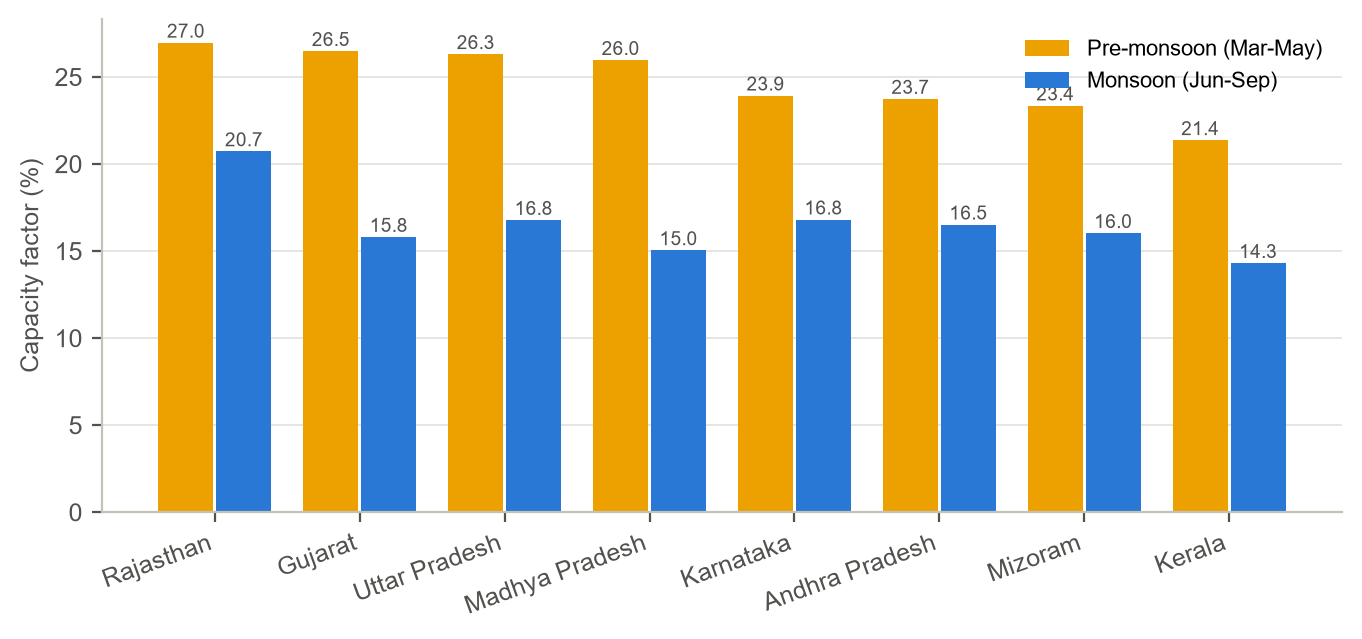
\includegraphics[width=0.8\textwidth]{seasonal_cf_state.png}
    \caption{Average simulated capacity factor of core parks by State: pre-monsoon vs monsoon (2025).}
    \label{fig:seasonal}
\end{figure}

Looking at individual weeks at Bhadla-II, in January the output closely follows the clear-sky curve. In July several days are strongly reduced by cloud, with large hour-to-hour changes. These are exactly the conditions under which forecasting is hardest.


\section{Accuracy of Weather Forecasts}
\vspace{1mm}
Because model inputs are ECMWF forecasts issued a day earlier, their accuracy sets a realistic limit on how well generation can be forecast. We compared the day-1 GHI forecast with ERA5 in daylight hours at all 36 locations (about 10,400 hours each). Figure~\ref{fig:nwpbias} summarises the results by State.

\begin{figure}[htbp]
    \centering
    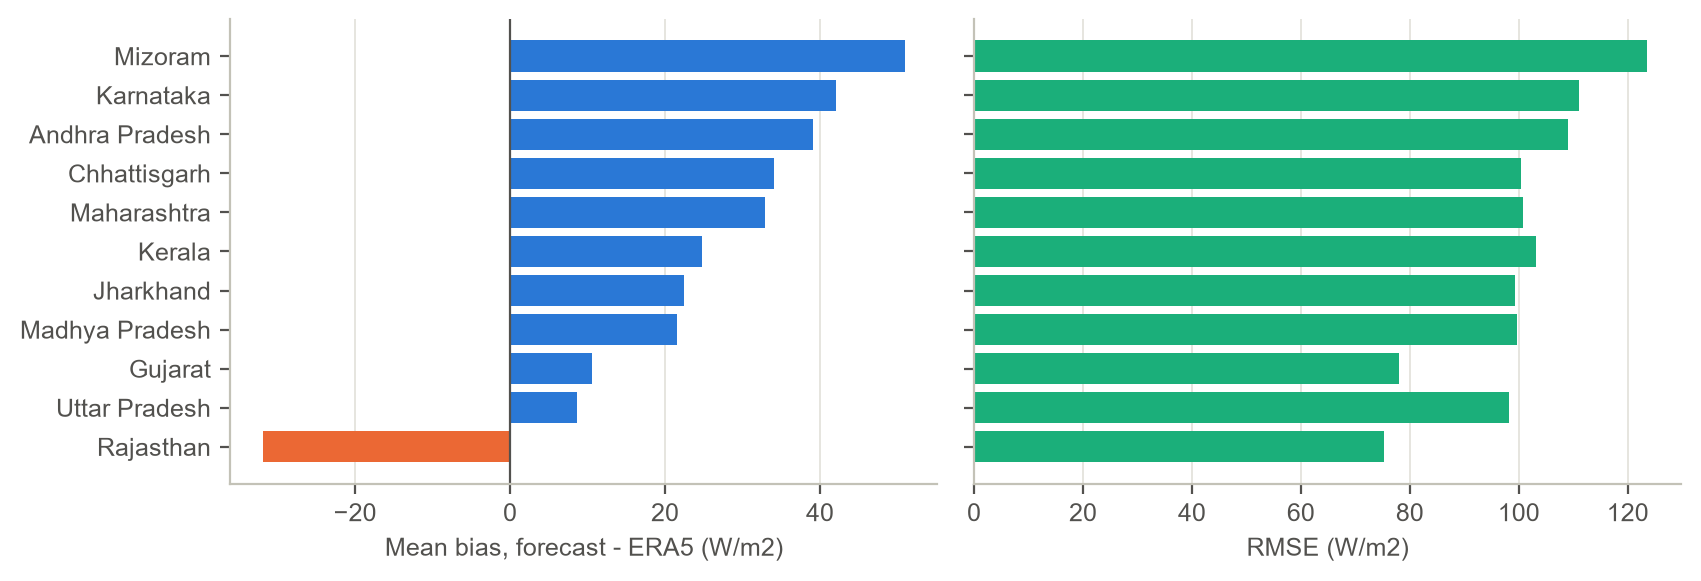
\includegraphics[width=0.85\textwidth]{nwp_bias_state.png}
    \caption{Mean bias and RMSE of the ECMWF day-1 GHI forecast by State.}
    \label{fig:nwpbias}
\end{figure}

\begin{figure}[htbp]
    \centering
    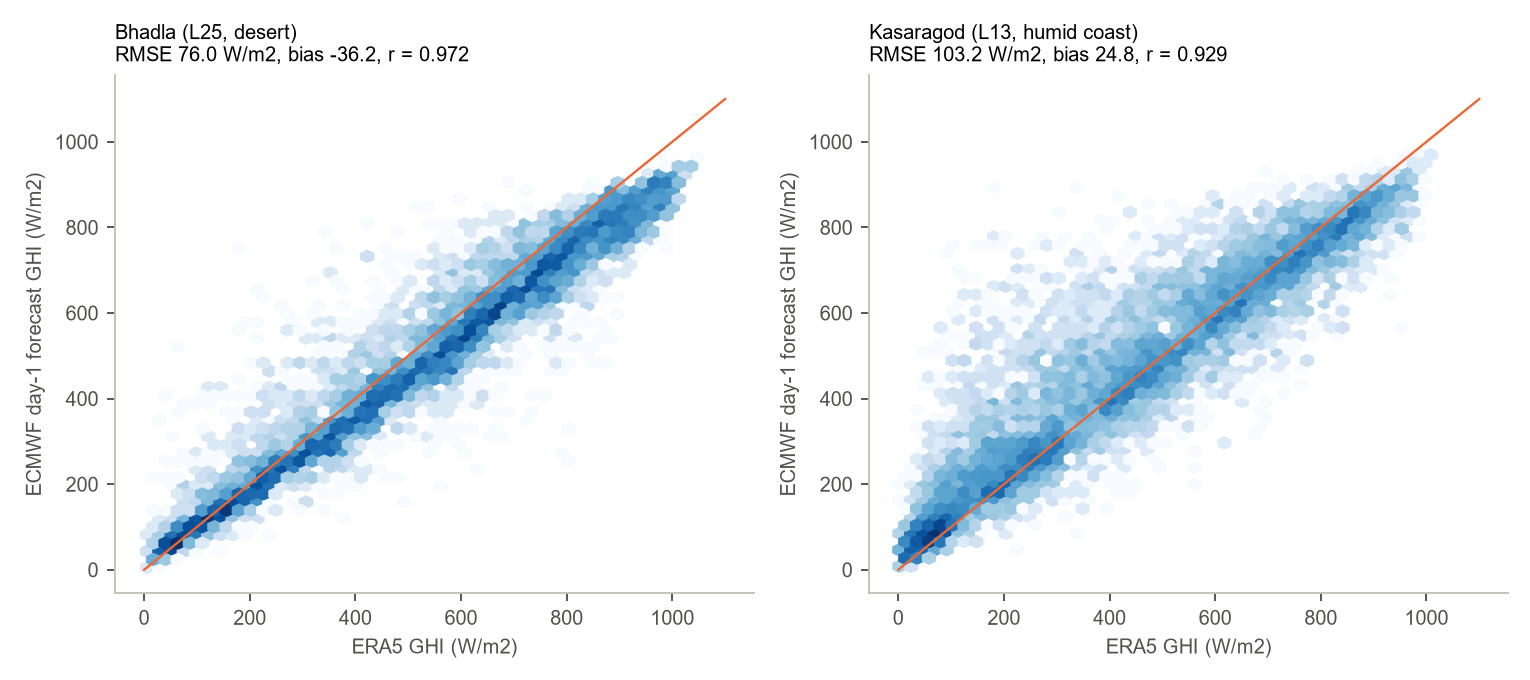
\includegraphics[width=0.8\textwidth]{fig_nwp_vs_era5.png}
    \caption{Day-1 forecast GHI against ERA5 GHI at a desert site (Bhadla) and a humid coastal site (Kasaragod).}
    \label{fig:nwpscatter}
\end{figure}

The forecasts are informative everywhere, with correlation between 0.90 and 0.97 and RMSE between 70 and 124~W/m$^2$. Two patterns stand out:
\begin{itemize}[noitemsep]
    \item \textbf{Regional bias with opposite signs.} The forecast \textit{under-estimates} GHI in Rajasthan (about $-30$ to $-37$~W/m$^2$) but \textit{over-estimates} it in southern and central India (about $+20$ to $+42$~W/m$^2$), and most strongly in Mizoram ($+51$~W/m$^2$). A likely reason is the different treatment of aerosols and dust in the forecast model and the reanalysis. Since the bias depends on the location, a global model needs location information to correct it. This supports including park metadata as features.
    \item \textbf{Accuracy follows climate.} Desert and Kutch sites have the lowest errors (nRMSE about 14--17\%), while monsoon-affected and hilly sites have the highest (about 24--30\%). We therefore expect the generation forecasts to be hardest in central and north-eastern India.
\end{itemize}

\section{Discussion}
\vspace{1mm}
The pipeline has produced a complete, clean and well-documented dataset for 43 parks. The simulation results are physically sensible: output is zero at night, never exceeds capacity, and responds correctly to clouds, seasons and temperature. The capacity factors are consistent with high-irradiance, ground-mounted Indian PV, but they are on an AC basis with assumed design parameters, so they should be compared in shape, not in level, with published utilisation factors until measured data are available. The forecast assessment shows that day-old NWP forecasts are useful but biased in a location-dependent way. This is exactly the error a machine-learning model can learn to correct.

% ================================================================ 8
\chapter{Forecasting Results}
This chapter presents the results of the eleven experiments. All numbers are measured on the test period (January--September 2026), which no model saw during training, over the daylight hours of all 43 parks. Errors are given as nRMSE in percent of park capacity (lower is better). The ``actual'' output is the simulated output described in Chapter~7, except in experiment E11, which uses measured data.

\section{Model Comparison (E1)}
\vspace{1mm}
Table~\ref{tab:e1} and Figure~\ref{fig:e1} compare all models at the four horizons.

\begin{table}[htbp]
\centering
\caption{Model comparison: nRMSE (\% of capacity), test period, all 43 parks.}
\label{tab:e1}
\begin{tabular}{lrrrr}
\toprule
Model & 1 h & 3 h & 6 h & 24 h \\
\midrule
Persistence & 14.80 & 36.81 & 52.51 & 9.68 \\
Climatology & 9.82 & 9.82 & 9.82 & 9.82 \\
Smart persistence (main baseline) & 5.28 & 9.09 & 11.61 & 9.79 \\
ECMWF forecast + physics & 8.61 & 8.61 & 8.61 & 8.78 \\
Ridge regression & 4.95 & 6.53 & 6.88 & 7.18 \\
Random Forest & 4.50 & 5.99 & 6.49 & 7.00 \\
XGBoost (GPU) & 4.50 & 5.99 & 6.54 & 7.09 \\
LightGBM & 4.53 & 6.02 & 6.59 & 7.10 \\
LSTM (GPU) & 4.53 & 6.05 & 6.57 & 7.09 \\
GRU (GPU) & 4.52 & 6.07 & 6.59 & 7.06 \\
\textbf{LightGBM + GRU average} & \textbf{4.47} & \textbf{5.98} & \textbf{6.52} & \textbf{7.02} \\
\midrule
Skill vs smart persistence & 15\% & 34\% & 44\% & 28\% \\
\bottomrule
\end{tabular}
\end{table}

\begin{figure}[htbp]
    \centering
    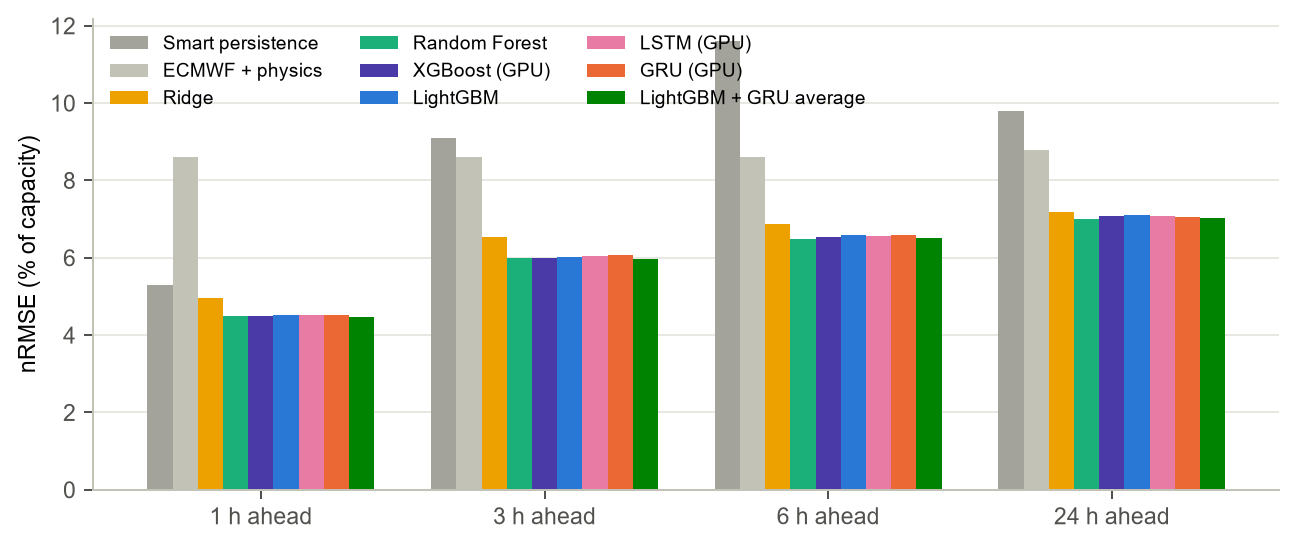
\includegraphics[width=0.95\textwidth]{fig_e1_models.png}
    \caption{nRMSE of all models at 1, 3, 6 and 24 hours ahead.}
    \label{fig:e1}
\end{figure}

\begin{itemize}[noitemsep]
    \item \textbf{Every learned model beats every baseline.} The gain over smart persistence grows with the horizon, from 15\% at 1 hour to 44\% at 6 hours, because recent output says less about the future the further ahead we look, while the weather forecast stays useful.
    \item \textbf{The learned models are very close to each other.} Random Forest, XGBoost, LightGBM, LSTM and GRU are within about 0.1 percentage points. The information in the inputs, not the type of model, limits accuracy. Averaging LightGBM and GRU gives a small further gain.
    \item \textbf{Combining physics and learning helps.} The ECMWF forecast passed through the physical model alone gives 8.6\%. Machine learning corrects its location-dependent bias and adds recent output, and reduces the error by about a quarter at day-ahead.
    \item \textbf{Tuning gives little (E10).} CatBoost on the GPU and a tuned LightGBM both reach 4.49 / 6.00 / 6.54\% at 1 / 3 / 6 hours, only 0.04--0.05 points better than the default LightGBM.
\end{itemize}

\begin{figure}[htbp]
    \centering
    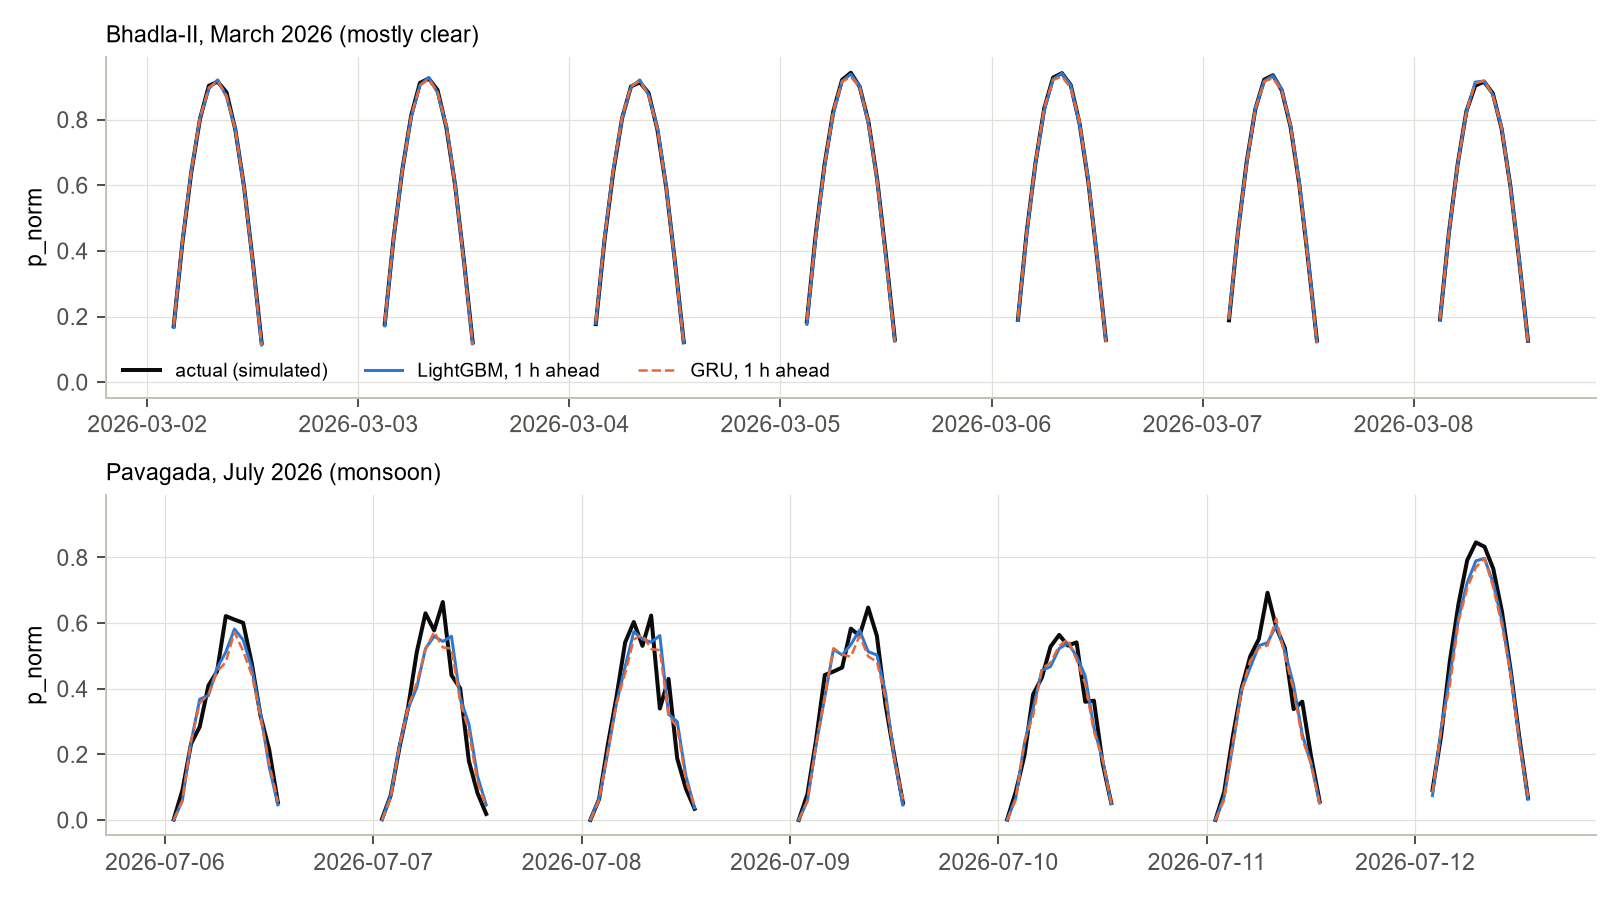
\includegraphics[width=0.95\textwidth]{fig_example_forecasts.png}
    \caption{1-hour-ahead forecasts against actual output: a clear week at Bhadla-II and a monsoon week at Pavagada.}
    \label{fig:examples}
\end{figure}

Figure~\ref{fig:examples} shows typical forecasts. On clear days the forecast is almost perfect. In the monsoon the models follow the general shape but cannot predict every short cloud-driven dip.

\section{Multi-Site Designs (E2, E3)}
\vspace{1mm}
\begin{table}[htbp]
\centering
\caption{One global model against separate models (nRMSE \%, LightGBM).}
\label{tab:e23}
\begin{tabular}{lrrrr}
\toprule
Design & Groups & 1 h & 3 h & 6 h \\
\midrule
One model per park (E2) & 43 & 4.67 & 6.19 & 6.72 \\
One global model, same parks & 1 & \textbf{4.43} & \textbf{5.92} & \textbf{6.48} \\
\midrule
One model per grid region (E3) & 5 & 5.35 & 6.89 & 7.49 \\
One global model, same parks & 1 & \textbf{5.21} & \textbf{6.74} & \textbf{7.36} \\
\midrule
One model per Köppen climate class & 8 & 4.53 & 6.02 & 6.55 \\
One model per weather cluster ($k=5$) & 5 & 4.51 & 6.00 & 6.54 \\
One global model, same parks & 1 & \textbf{4.45} & \textbf{5.94} & \textbf{6.50} \\
\bottomrule
\end{tabular}
\end{table}

The single global model wins in every comparison (Table~\ref{tab:e23}). It is better than the per-park model at 43 of 43 parks at 1 and 3 hours and at 42 of 43 parks at 6 hours. Climate grouping was tested in two objective ways. Each park was given its Köppen--Geiger class \cite{rubel2017} (14 hot semi-arid, 13 hot desert and six smaller classes), and the weather locations were also clustered by their monthly climate in the training period (k-means; $k=5$ had the best silhouette score, 0.45). The global model still beats the climate-group models in 8 of 8 Köppen groups and 5 of 5 clusters at 1 hour. A model that sees all parks learns more about clouds, seasons and forecast bias than a model that sees only a few similar parks.

\section{Which Inputs Matter (E4, E9)}
\vspace{1mm}
\begin{table}[htbp]
\centering
\caption{Input ablation (nRMSE \%) and SHAP share of each input group.}
\label{tab:e4}
\begin{tabular}{lrrr}
\toprule
 & 1 h & 3 h & 6 h \\
\midrule
All inputs & 4.53 & 6.02 & 6.59 \\
Without weather forecast & 4.66 & 6.65 & 7.80 \\
Without park metadata & 4.52 & 6.02 & 6.58 \\
Weather forecast and sun position only & 7.02 & 7.02 & 7.02 \\
\midrule
SHAP share: weather forecast & 54\% & 65\% & 71\% \\
SHAP share: recent output & 36\% & 24\% & 19\% \\
SHAP share: sun position and time & 8.6\% & 8.3\% & 7.4\% \\
SHAP share: park metadata & 1.1\% & 2.4\% & 2.8\% \\
\bottomrule
\end{tabular}
\end{table}

Both main input groups are needed (Table~\ref{tab:e4}). Recent output matters most at 1 hour; the weather forecast becomes more important as the horizon grows, and removing it raises the 6-hour error from 6.6\% to 7.8\%. Park metadata adds almost nothing, because the park identifier and the recent output already describe each park. If the model is given the weather that actually happened instead of the forecast (E9, an ``oracle'' test), the error falls to about 0.35\%. Almost all the remaining error therefore comes from the weather forecast, not from the model.

\section{Aggregation (E5)}
\vspace{1mm}
\begin{table}[htbp]
\centering
\caption{nRMSE (\% of capacity) at four aggregation levels (capacity-weighted).}
\label{tab:e5}
\begin{tabular}{lrrrr}
\toprule
Horizon & Park & State & Region & All parks \\
\midrule
1 h & 4.09 & 3.01 & 2.29 & 1.37 \\
3 h & 5.61 & 4.30 & 3.29 & 2.00 \\
6 h & 6.13 & 4.75 & 3.63 & 2.23 \\
24 h & 6.64 & 5.26 & 4.04 & 2.56 \\
\bottomrule
\end{tabular}
\end{table}

\begin{figure}[htbp]
    \centering
    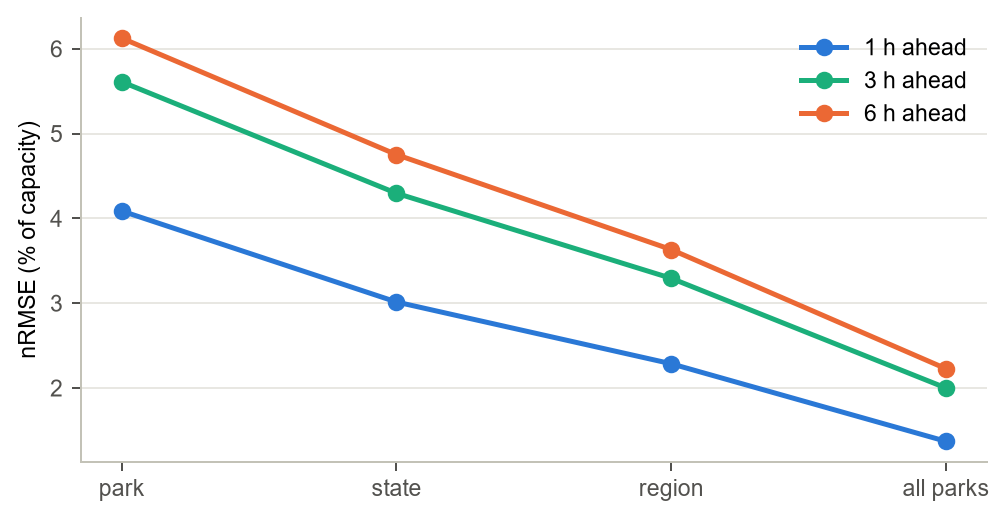
\includegraphics[width=0.7\textwidth]{fig_e5_aggregation.png}
    \caption{Forecast error falls as park forecasts are added up to State, region and all-park level.}
    \label{fig:e5}
\end{figure}

Adding forecasts together cuts the error by about two-thirds from park to all-park level (Table~\ref{tab:e5}, Figure~\ref{fig:e5}). The reason is that errors at distant parks are nearly independent: the correlation of forecast errors is 0.62 for parks within 100~km, 0.17 at 100--300~km, 0.02 at 300--600~km and about zero beyond. Errors at distant parks partly cancel, so forecasting a geographically spread portfolio is much easier than forecasting one park.

\section{Difficult Conditions (E6)}
\vspace{1mm}
At 1 hour the error is 3.2\% on clear days, 7.9\% on partly cloudy days and 6.7\% on overcast days; it is 6.3\% in the monsoon and 3.6\% outside it. Ramp hours (sudden changes in cloudiness, about 1\% of daylight hours) are much harder: the error is 21.8\% against 27.1\% for smart persistence, compared with 4.5\% in normal hours. The model reduces the size of ramp errors but cannot predict that a ramp will happen (probability of detection 0.04). Ramps caused by single clouds are smaller than the 25~km weather-forecast grid, so hourly forecasts cannot see them.

\section{Unseen Parks (E7)}
\vspace{1mm}
Each weather location was removed in turn, a model was trained on the others, and the removed parks were forecast. The extra error is small on average: $+0.37$ percentage points at 1 hour and $+0.63$ at 6 hours. The worst cases are parks with unusual climates (up to $+4.2$ points at 1 hour). A new park can therefore get useful forecasts on its first day, before it has any history of its own, provided its climate is represented in the training parks.

\section{Prediction Intervals (E8)}
\vspace{1mm}
\begin{table}[htbp]
\centering
\caption{Coverage of 80\% prediction intervals (target 80\%).}
\label{tab:e8}
\begin{tabular}{lrrrr}
\toprule
 & 1 h & 3 h & 6 h & 24 h \\
\midrule
Quantile LightGBM, raw & 69.7\% & 71.8\% & 73.3\% & 73.8\% \\
After conformal calibration (CQR) & 80.3\% & 81.2\% & 82.0\% & 82.1\% \\
Mean width, \% of capacity (CQR) & 7.8 & 10.9 & 12.1 & 13.2 \\
\midrule
All-parks total: coverage & 83.8\% & 83.8\% & 83.7\% & 83.9\% \\
All-parks total: $\pm$ half-width (MW) & 521 & 791 & 880 & 1,022 \\
\bottomrule
\end{tabular}
\end{table}

The raw quantile model is over-confident: its 80\% intervals contain the actual value only about 70\% of the time. After conformal calibration the coverage is 80--82\% at every horizon (Table~\ref{tab:e8}). Monthly coverage at 1 hour stays between 76\% and 85\%, slightly lower in the monsoon months. For the all-parks total, the 1-hour forecast is accurate to about $\pm$520~MW with 80\% confidence.

\section{Test on Real Measured Plants (E11)}
\vspace{1mm}
To check that results on simulated output carry over to real plants, we used a public dataset of two Indian solar plants with 15-minute measured output and on-site sensors (May--June 2020) \cite{kaggleplants}. First, the physical model was fed with each plant's measured irradiance and module temperature (Figure~\ref{fig:e11}). For Plant~1 the simulated output follows the measured output closely (correlation 0.992, error 3.4\% after calibration). For Plant~2 it fits less well (correlation 0.821, error 16.0\%), because of outages and partial shutdowns in the measured data that no weather model can explain.

\begin{figure}[htbp]
    \centering
    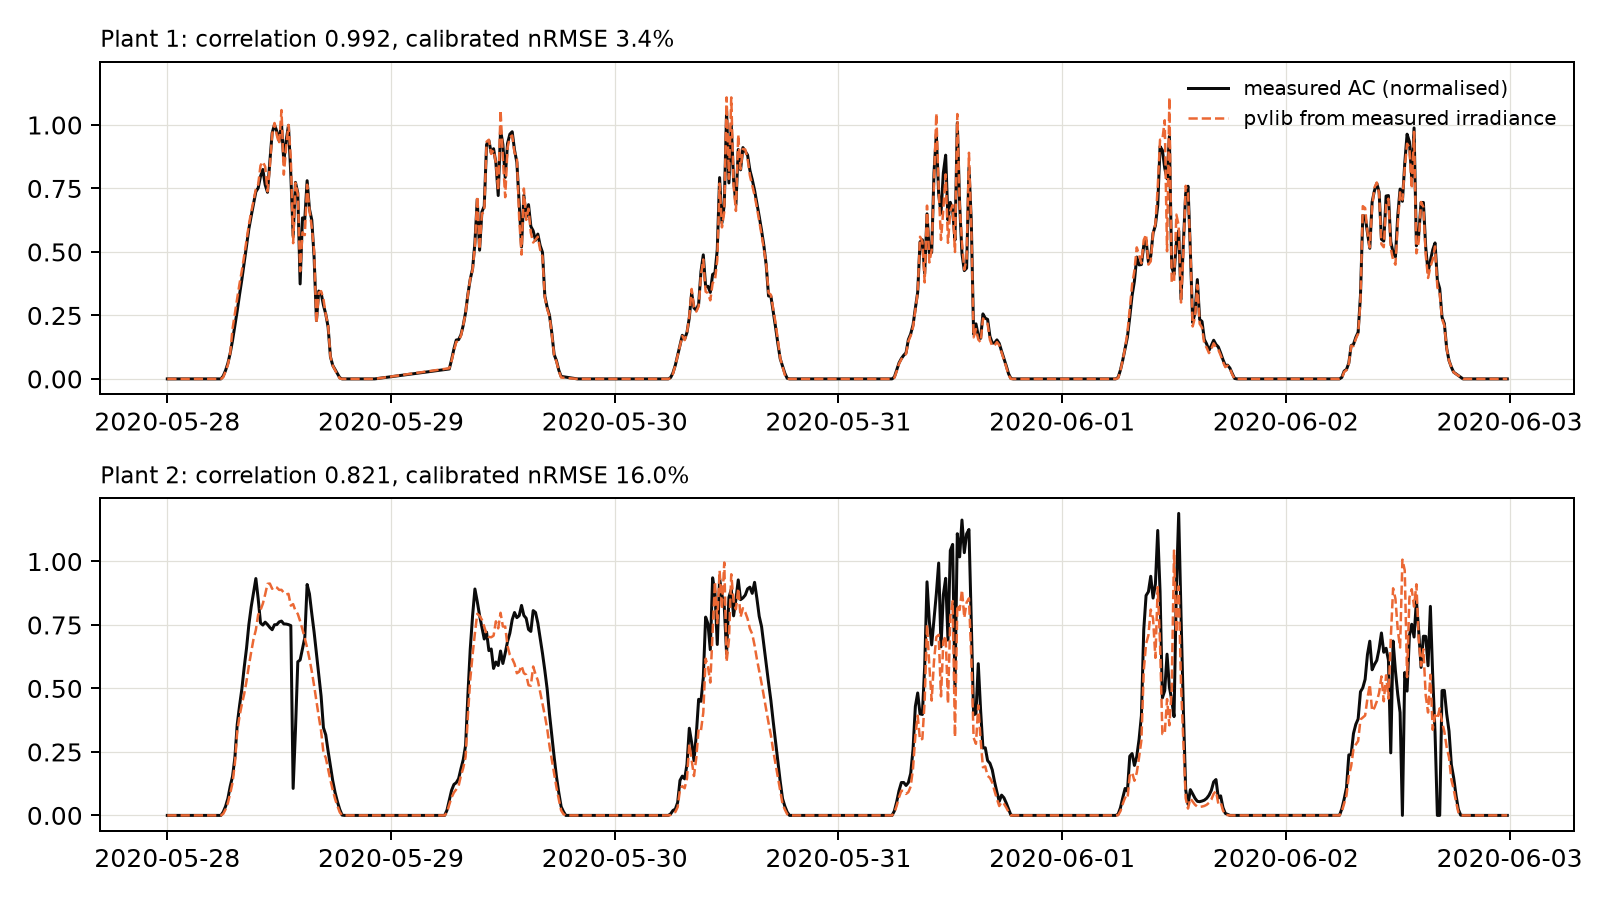
\includegraphics[width=0.95\textwidth]{fig_e11_real.png}
    \caption{Measured output of two real Indian plants against the \texttt{pvlib} simulation from measured irradiance.}
    \label{fig:e11}
\end{figure}

\begin{table}[htbp]
\centering
\caption{Forecasting real measured output (nRMSE \%).}
\label{tab:e11}
\begin{tabular}{lrrrr}
\toprule
 & \multicolumn{2}{c}{Plant 1} & \multicolumn{2}{c}{Plant 2} \\
Model & 1 h & 3 h & 1 h & 3 h \\
\midrule
Persistence & 17.26 & 37.16 & 17.44 & 29.82 \\
Smart persistence & 11.15 & 15.87 & 13.44 & 18.06 \\
Trained only on the plant's own data & 11.75 & 14.03 & 12.93 & 14.09 \\
Our model, no retraining & 10.25 & \textbf{12.42} & 12.57 & 14.60 \\
Our model, fine-tuned on the plant & \textbf{10.15} & 13.69 & \textbf{11.84} & 14.48 \\
\bottomrule
\end{tabular}
\end{table}

Second, we forecast the measured output (Table~\ref{tab:e11}). The model trained only on our simulated parks, with no retraining, beats smart persistence at both plants and both horizons, and it is better than a model trained on the plant's own short history in three of four cases. Fine-tuning on the plant's data helps a little at 1 hour. Errors are higher than on simulated output, as expected for real plants with outages, soiling and sensor noise, but the main finding holds: knowledge learned from simulated parks transfers to real ones.

\section{Discussion}
\vspace{1mm}
The results answer the research questions clearly. Machine learning that combines recent output with archived weather forecasts beats all standard baselines at every horizon. One global model is better than per-park, regional or climate-group models, and it generalises to unseen parks. Aggregation strongly reduces error, calibrated intervals are reliable, and the approach transfers to measured data. The main limit is the weather forecast itself: with perfect weather information the error would be more than ten times smaller. Better forecasts, for example satellite-based nowcasts, are therefore the most promising route to further improvement.

% ================================================================ 9
\chapter{Dashboard, API and Public Website}
The forecasts are made available in three ways: a Python API for other programs, an interactive dashboard for analysts, and a public website that anyone can open. All three read the same saved test-period forecasts.

\section{Forecast API}
\vspace{1mm}
A FastAPI service provides four endpoints: \texttt{/parks} (list of parks with location and capacity), \texttt{/forecast/park/\{id\}} (forecast in MW with its 80\% interval for one park), \texttt{/forecast/total} (State, region or all-park totals) and \texttt{/metrics} (model accuracy by horizon). The horizon (1, 3, 6 or 24 hours) and the time range are query parameters, and invalid requests are rejected with clear messages. Interactive documentation is generated automatically.

\section{Dashboard}
\vspace{1mm}
A Streamlit dashboard offers four pages: an India map with one marker per park (size shows capacity, colour shows error); a park explorer showing actual output, the forecast and its interval; State, region and all-park totals; and the experiment results. The user chooses the horizon and the date range.

\section{Public Website}
\vspace{1mm}
To make the project accessible without installing anything, we built a static website and published it on GitHub Pages:\\
\texttt{https://navneet-cerecode.github.io/mnre-solar-forecast/}\\

The website has an SVG map of India with State boundaries and all 43 parks, a park explorer with forecast charts, aggregated totals with intervals, and a results section (Figures~\ref{fig:web1} and~\ref{fig:web2}). Charts are drawn with Chart.js. To keep the site fast, the forecasts for all parks and horizons are packed into compact files (about one byte per value). The site works on phones and does not need a server.

\begin{figure}[htbp]
    \centering
    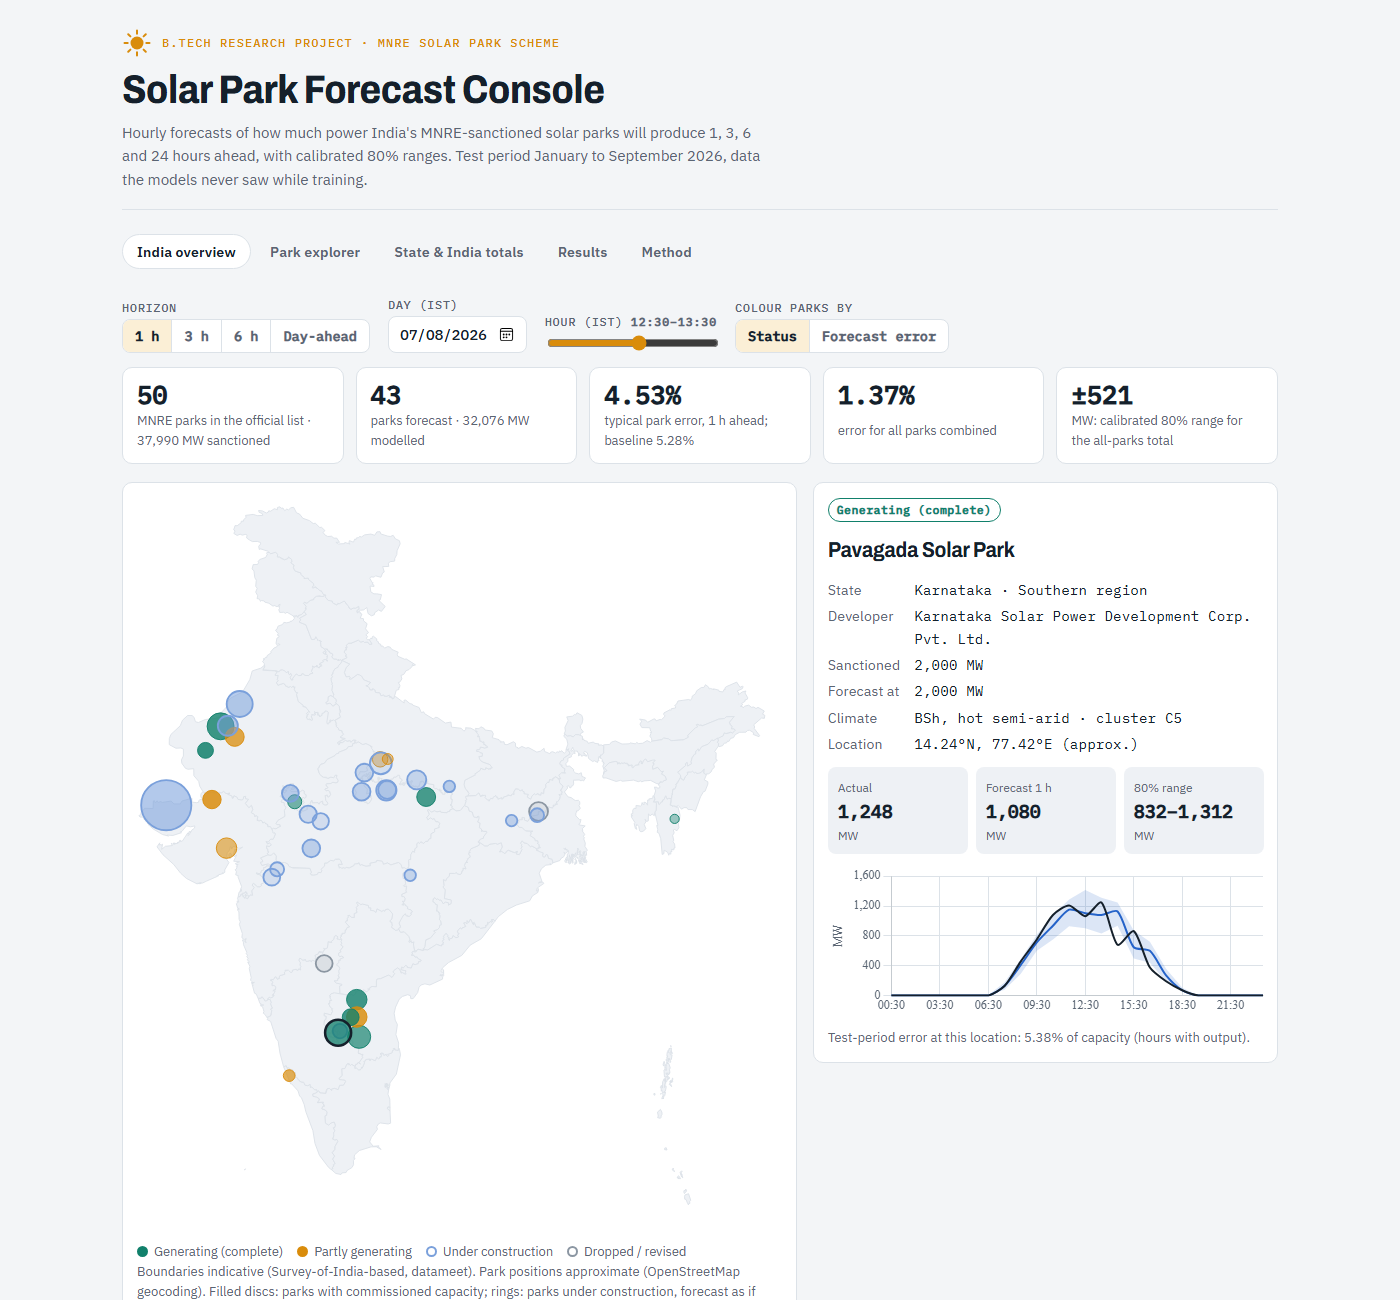
\includegraphics[width=0.9\textwidth]{website_overview.png}
    \caption{Public website: India map and park explorer.}
    \label{fig:web1}
\end{figure}

\begin{figure}[htbp]
    \centering
    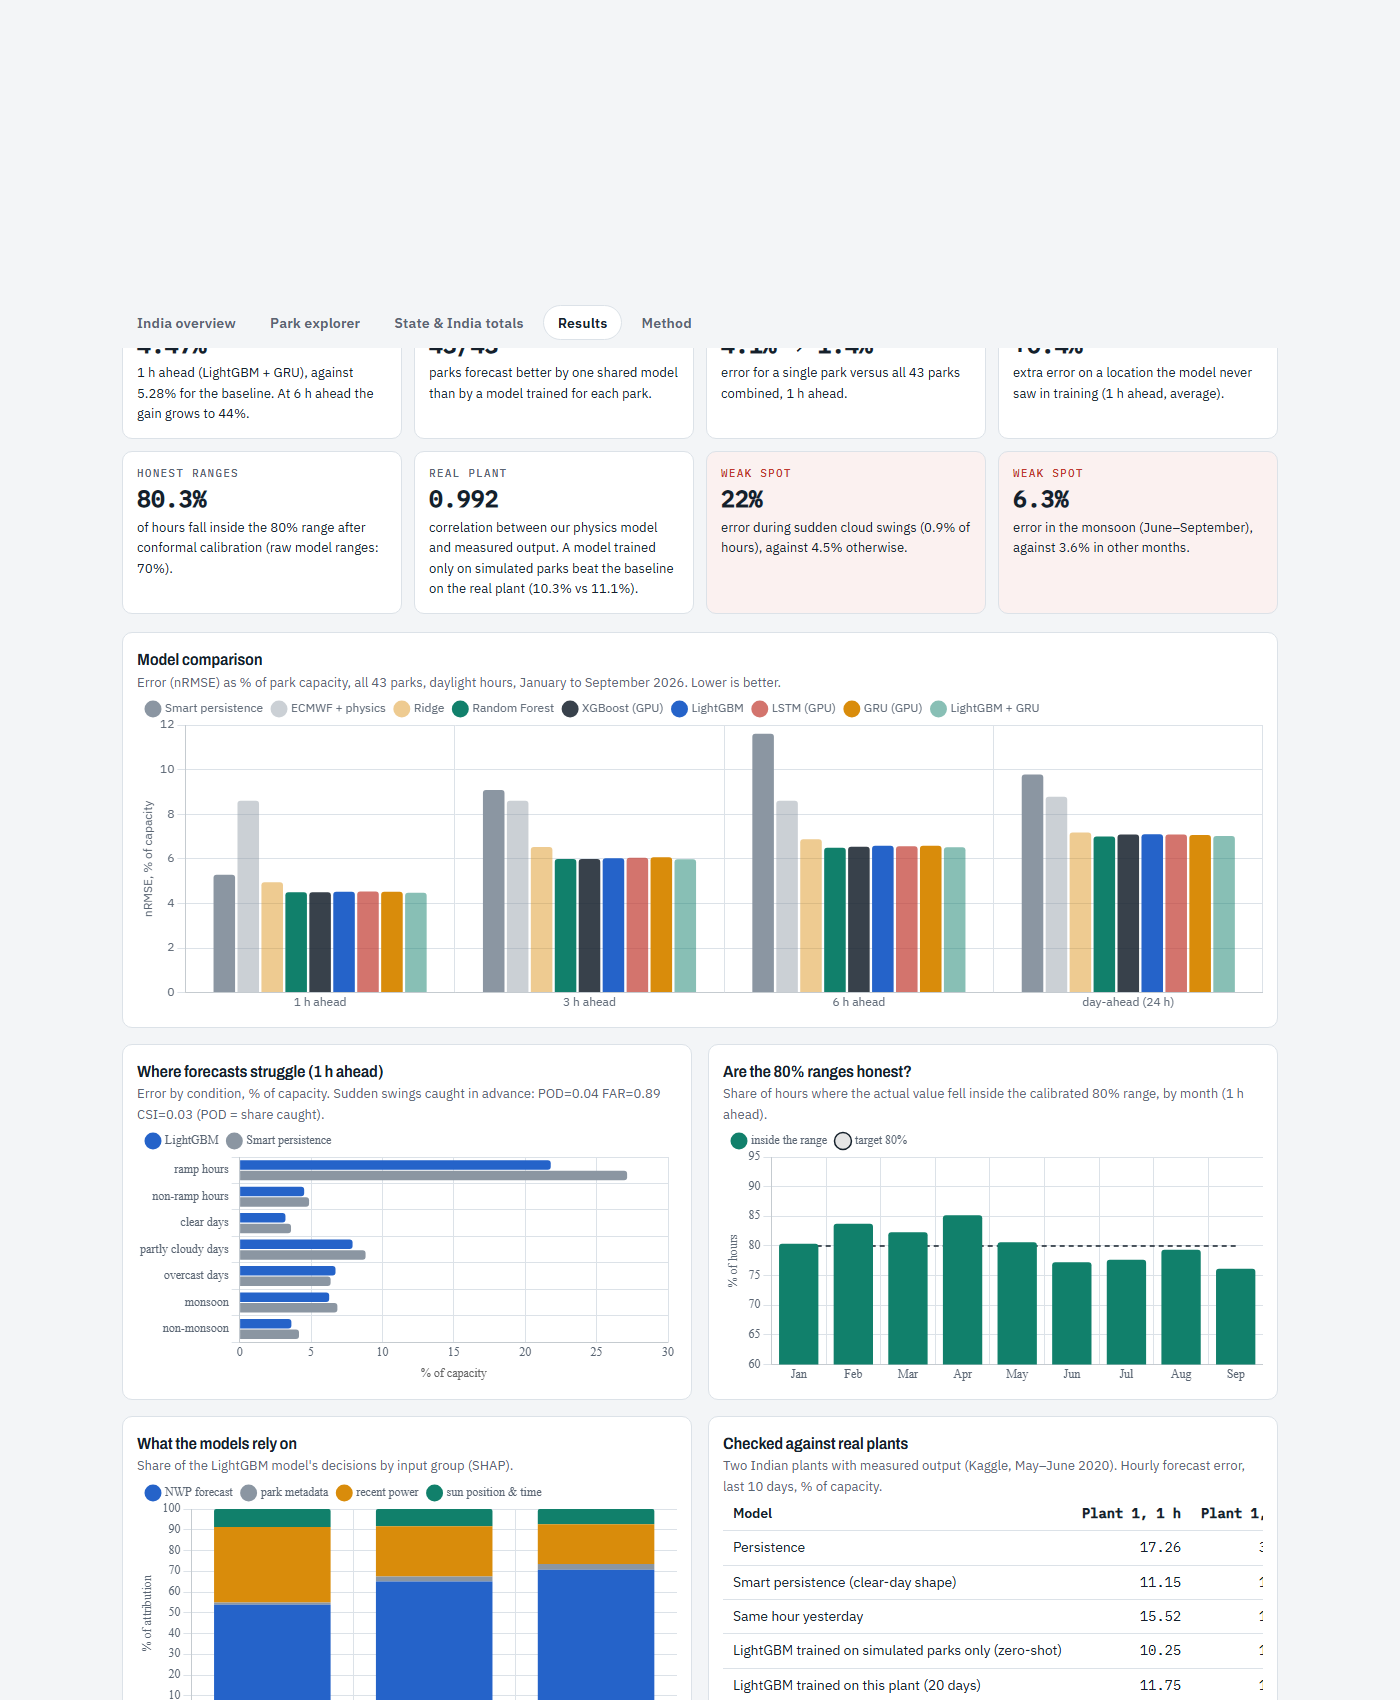
\includegraphics[width=0.9\textwidth]{website_results.png}
    \caption{Public website: aggregated forecast and results.}
    \label{fig:web2}
\end{figure}

% ================================================================ 9
\chapter{Challenges, Limitations and Future Scope}
\section{Technical Challenges}
\vspace{1mm}
\begin{itemize}[noitemsep]
    \item \textbf{No public measured generation:} the main risk is forecasting a simulation. It is mitigated by separating forecast inputs from observed-weather targets, labelling all results clearly, and testing on measured data wherever possible.
    \item \textbf{Unknown plant design:} tilt, trackers, DC/AC ratio and module type are not published per park.
    \item \textbf{Time-varying capacity:} commissioning after October 2023 is not published park by park.
    \item \textbf{Coarse weather grids:} 25~km cells smooth cloud edges, and several parks share a cell.
    \item \textbf{Monsoon and aerosols:} forecast errors are largest exactly when output is most variable.
    \item \textbf{Inaccessible government websites:} several official portals could not be reached during research, so some records were obtained from mirrors.
\end{itemize}

\section{Risk Mitigation}
\vspace{1mm}
\begin{table}[htbp]
\centering
\caption{Risk register.}
\label{tab:risk}
\begin{tabularx}{\textwidth}{p{4.3cm}p{1.6cm}L}
\toprule
Risk & Likelihood & Mitigation \\
\midrule
No measured park data obtained & High & Hybrid target; Kaggle Indian plants for sim-to-real checks; request data through the guide \\
Wrong simulation assumptions & Medium & Sensitivity analysis; calibration against published annual energy \\
Leakage between targets and features & Medium & Separate data sources; lead-time rule; leakage checklist \\
Change of data-service terms & Low & All raw downloads cached; ERA5 also available from Copernicus \\
Deep learning does not beat LightGBM & Medium & Report honestly; the comparison is itself a result \\
Schedule slip & Medium & Core experiments first; weekly milestones \\
\bottomrule
\end{tabularx}
\end{table}

\section{Limitations}
\vspace{1mm}
\begin{itemize}[noitemsep]
    \item The park-wise composition of the historical 42-park set is not verified; the master universe is the 2023 official list.
    \item Most targets are simulated and describe weather-driven potential output, not real operational output.
    \item Coordinates are approximate, and some parks span several sites.
    \item Hourly resolution under-represents sub-hourly cloud variability, while Indian scheduling uses 15-minute blocks.
    \item Reanalysis ``observed'' weather is itself a model product with its own irradiance errors.
    \item The real-data test (E11) covers only two plants and 34 days, without archived weather forecasts for that period.
    \item The Köppen map places seven central-Indian parks in a ``Mediterranean'' class, which is an artefact of the coarse climate map.
    \item The dashboard and website show saved test-period forecasts; they are not yet connected to live weather forecasts.
\end{itemize}

\section{Future Scope}
\vspace{1mm}
\begin{itemize}[noitemsep]
    \item Spatio-temporal graph neural networks, if measured data become available at enough parks.
    \item Satellite-based nowcasting (INSAT-3D/3DR, Meteosat) for 0--2 hour horizons, the most promising route since most remaining error comes from the weather forecast (E9) and ramps are not detected (E6).
    \item Running the system live: download each new ECMWF forecast automatically and update the website every hour.
    \item Adaptive conformal intervals that adjust to the monsoon, where coverage currently dips to about 76\%.
    \item Larger deep-learning models (Temporal Fusion Transformer, N-HiTS) and a blend of several weather models.
    \item 15-minute forecasts aligned with Indian scheduling and deviation settlement.
    \item Hierarchical probabilistic reconciliation across aggregation levels.
    \item Extension to all solar plants in a State using load-despatch data, and to hybrid wind--solar parks.
    \item Collaboration with a park developer or load-despatch centre to test the system live.
\end{itemize}

% ================================================================ 10
\clearpage
\chapter{Conclusion}
In this project we turned a single-plant forecasting idea into an India-wide research study of the MNRE-sanctioned solar parks. We verified the study universe from official records. The commonly quoted figure of 42 parks (23,499~MW) is correct for March 2019, but the official count has since changed, and the latest park-wise list contains 50 parks with 37,990~MW, which we documented in a source-cited master table.\\

Because no park publishes hourly generation, we designed a hybrid approach that simulates generation with a physical PV model and keeps model inputs (archived forecasts) strictly separate from the weather used to build targets. We implemented and tested the full data pipeline, which produced a complete dataset for 43 parks at 36 locations from April 2024 to September 2026 with no missing values.\\

We then trained baseline, machine-learning and deep-learning models, using the GPU for XGBoost, CatBoost, LSTM and GRU, and ran eleven experiments on an unseen test period. A single global model reduces the error of smart persistence by 15\% at 1 hour, 34\% at 3 hours, 44\% at 6 hours and 28\% day-ahead. The different learned models perform almost equally, so the inputs matter more than the algorithm. One global model beats per-park, grid-region and climate-zone models and works for unseen parks. Adding forecasts across India cuts the error by about two-thirds, because errors at distant parks are nearly independent. Conformal calibration turns over-confident intervals into reliable 80\% intervals. Most importantly, a model trained only on simulated parks beats smart persistence on two real Indian plants without retraining.\\

The forecasts are available through an API, a dashboard and a public website. The remaining error comes mainly from the weather forecast and from sudden cloud ramps, which points to satellite nowcasting and live operation as the next steps. We believe the project provides an honest and useful benchmark for short-term solar forecasting in India.

% ================================================================ Appendix
% ================================================================ References
\clearpage
\addcontentsline{toc}{chapter}{Bibliography}
\begingroup
\small
\begin{thebibliography}{99}
\setlength{\itemsep}{0pt}\setlength{\parsep}{0pt}
\bibitem{ls3633} Ministry of New and Renewable Energy, ``Development of Solar Parks'', Lok Sabha Unstarred Question No.~3633, answered 10.08.2023 (Annexure: park-wise sanctioned capacity).
\bibitem{seci2019} Solar Energy Corporation of India, \textit{8th Annual Report 2018--19}, Directors' Report, Sec.~IV ``Solar Parks Scheme''. [Online]. Available: \texttt{https://www.seci.co.in}.
\bibitem{pib145542} Press Information Bureau, ``Fact Sheet on Scheme for Development of Solar Parks and Ultra Mega Solar Power Projects'', MNRE, 23 May 2016.
\bibitem{pib158621} Press Information Bureau, ``Cabinet approves enhancement of capacity from 20,000~MW to 40,000~MW of the Scheme for Development of Solar Parks and Ultra Mega Solar Power Projects'', 2017.
\bibitem{pibyer2018} Press Information Bureau, ``Year End Review 2018 -- MNRE'', 10 December 2018.
\bibitem{pibyer2020} Press Information Bureau, ``MNRE: Year End Review 2020''.
\bibitem{pib1809373} Press Information Bureau, ``Government implements schemes to set up 50 Solar Parks of aggregate capacity 40,000~MW'', 24 March 2022.
\bibitem{pib1883116} Press Information Bureau, ``Status of Solar and Ultra Mega Solar power projects'', 13 December 2022.
\bibitem{pib1907702} Press Information Bureau, ``Establishment of Solar Parks'', 16 March 2023.
\bibitem{pib1909951} Press Information Bureau, ``Eight Solar Parks with aggregate capacity of 4995~MW approved in Bundelkhand region'', 23 March 2023.
\bibitem{pib1941144} Press Information Bureau, ``11 Solar Parks with 8521~MW capacity completed and 7 Solar Parks partially completed'', Lok Sabha Q.145, 20 July 2023.
\bibitem{pib1983203} Press Information Bureau, ``50 Solar Parks of nearly 37.5~GW sanctioned since 2014; capacity of 10.2~GW established'', 6 December 2023.
\bibitem{rs2851} Rajya Sabha Unstarred Question No.~2851 (Session 267), answered 25.03.2025, Open Government Data Platform India. [Online]. Available: \texttt{https://data.gov.in}.
\bibitem{pib2199729} Press Information Bureau, ``India's Solar Momentum'' (Backgrounder), 6 December 2025.
\bibitem{pibnote2026} Press Information Bureau, ``India's Solar Growth Enters a New Era'' (Press Note), 2 August 2026.
\bibitem{cerc2015} Central Electricity Regulatory Commission, ``Framework on Forecasting, Scheduling and Deviation Settlement of Wind and Solar Generating Stations at the Inter-State Level'', 2015.
\bibitem{era5} H. Hersbach \textit{et al.}, ``The ERA5 global reanalysis'', \textit{Quarterly Journal of the Royal Meteorological Society}, vol.~146, pp.~1999--2049, 2020.
\bibitem{era5land} J. Muñoz-Sabater \textit{et al.}, ``ERA5-Land: a state-of-the-art global reanalysis dataset for land applications'', \textit{Earth System Science Data}, vol.~13, pp.~4349--4383, 2021.
\bibitem{openmeteo} Open-Meteo, ``Historical Weather API and Previous Runs API documentation''. [Online]. Available: \texttt{https://open-meteo.com}. [Accessed: Oct-2026].
\bibitem{nasapower} NASA, ``Prediction of Worldwide Energy Resources (POWER)''. [Online]. Available: \texttt{https://power.larc.nasa.gov}.
\bibitem{cams} Copernicus Atmosphere Monitoring Service, ``CAMS solar radiation time-series''. [Online]. Available: \texttt{https://ads.atmosphere.copernicus.eu}.
\bibitem{pvlib} W. F. Holmgren, C. W. Hansen and M. A. Mikofski, ``pvlib python: a python package for modeling solar energy systems'', \textit{Journal of Open Source Software}, vol.~3, no.~29, p.~884, 2018.
\bibitem{pvwatts} A. P. Dobos, ``PVWatts Version 5 Manual'', NREL/TP-6A20-62641, 2014.
\bibitem{perez1990} R. Perez \textit{et al.}, ``Modeling daylight availability and irradiance components from direct and global irradiance'', \textit{Solar Energy}, vol.~44, no.~5, pp.~271--289, 1990.
\bibitem{beck2018} H. E. Beck \textit{et al.}, ``Present and future Köppen-Geiger climate classification maps at 1-km resolution'', \textit{Scientific Data}, vol.~5, 180214, 2018.
\bibitem{antonanzas2016} J. Antonanzas \textit{et al.}, ``Review of photovoltaic power forecasting'', \textit{Solar Energy}, vol.~136, pp.~78--111, 2016.
\bibitem{yang2018} D. Yang, J. Kleissl, C. A. Gueymard, H. T. C. Pedro and C. F. M. Coimbra, ``History and trends in solar irradiance and PV power forecasting'', \textit{Solar Energy}, vol.~168, pp.~60--101, 2018.
\bibitem{breiman2001} L. Breiman, ``Random forests'', \textit{Machine Learning}, vol.~45, pp.~5--32, 2001.
\bibitem{xgboost} T. Chen and C. Guestrin, ``XGBoost: a scalable tree boosting system'', in \textit{Proc. KDD}, 2016, pp.~785--794.
\bibitem{lightgbm} G. Ke \textit{et al.}, ``LightGBM: a highly efficient gradient boosting decision tree'', in \textit{Advances in Neural Information Processing Systems 30}, 2017.
\bibitem{lstm} S. Hochreiter and J. Schmidhuber, ``Long short-term memory'', \textit{Neural Computation}, vol.~9, no.~8, pp.~1735--1780, 1997.
\bibitem{gru} K. Cho \textit{et al.}, ``Learning phrase representations using RNN encoder-decoder for statistical machine translation'', in \textit{Proc. EMNLP}, 2014.
\bibitem{tft} B. Lim, S. O. Arik, N. Loeff and T. Pfister, ``Temporal Fusion Transformers for interpretable multi-horizon time series forecasting'', \textit{International Journal of Forecasting}, vol.~37, no.~4, pp.~1748--1764, 2021.
\bibitem{nhits} C. Challu \textit{et al.}, ``N-HiTS: neural hierarchical interpolation for time series forecasting'', in \textit{Proc. AAAI}, 2023.
\bibitem{hoff2010} T. E. Hoff and R. Perez, ``Quantifying PV power output variability'', \textit{Solar Energy}, vol.~84, no.~10, pp.~1782--1793, 2010.
\bibitem{koenker1978} R. Koenker and G. Bassett, ``Regression quantiles'', \textit{Econometrica}, vol.~46, no.~1, pp.~33--50, 1978.
\bibitem{romano2019} Y. Romano, E. Patterson and E. Candès, ``Conformalized quantile regression'', in \textit{Advances in Neural Information Processing Systems 32}, 2019.
\bibitem{gibbs2021} I. Gibbs and E. Candès, ``Adaptive conformal inference under distribution shift'', in \textit{Advances in Neural Information Processing Systems 34}, 2021.
\bibitem{shap} S. M. Lundberg and S.-I. Lee, ``A unified approach to interpreting model predictions'', in \textit{Advances in Neural Information Processing Systems 30}, 2017.
\bibitem{kaggleplants} A. Kannal, ``Solar Power Generation Data'' (two Indian plants, 34 days, 15-minute generation and sensor data), Kaggle, 2020. [Online]. Available: \texttt{https://www.kaggle.com/datasets/anikannal/solar-power-generation-data}.
\bibitem{rubel2017} F. Rubel, K. Brugger, K. Haslinger and I. Auer, ``The climate of the European Alps: shift of very high resolution Köppen-Geiger climate zones 1800--2100'', \textit{Meteorologische Zeitschrift}, vol.~26, no.~2, pp.~115--125, 2017 (used through the \texttt{kgcpy} package).
\bibitem{catboost} L. Prokhorenkova \textit{et al.}, ``CatBoost: unbiased boosting with categorical features'', in \textit{Advances in Neural Information Processing Systems 31}, 2018.
\end{thebibliography}
\endgroup

\end{document}
